% !TeX program = lualatex
\documentclass[a4paper]{article}
\usepackage{fontspec}
\usepackage{lmodern}
\usepackage[expansion=false]{microtype}
\usepackage{lastpage}
\usepackage[vietnamese,english]{babel}
\usepackage{textcomp}
\usepackage{ragged2e}
\usepackage{parskip}
\usepackage{float}
\usepackage{a4wide,amssymb,epsfig,latexsym,multicol,array,hhline,fancyhdr}
\usepackage{amsmath}
\usepackage[lined,boxed,commentsnumbered]{algorithm2e}
\usepackage{enumerate}
\usepackage{xcolor}
\usepackage{graphicx}
\usepackage{array}
\usepackage{tabularx, caption}
\usepackage{wrapfig}
\usepackage{multirow}
\usepackage{multicol}
\usepackage{rotating}
\usepackage{graphics}
\usepackage{geometry}
\usepackage{setspace}
\usepackage{epsfig}
\usepackage{tikz}
\usepackage{xfrac}
\usepackage{bm}
\usepackage{longtable}
\usepackage{listings}
\usepackage{placeins}
\usepackage{algorithm}
\usepackage{algpseudocode}
\usepackage[colorlinks]{hyperref}
\usepackage{tcolorbox}
\usepackage{caption}
\usepackage{makecell}
\usepackage{booktabs}
\usepackage{pifont}
\usepackage{subcaption}
\usepackage{calc}
\usepackage{enumitem}
\usepackage[sort=none,abbreviations,symbols,stylemods,style=list,nogroupskip,nonumberlist,nomain]{glossaries-extra}
\usepackage[backend=biber,style=numeric,sorting=none]{biblatex}
\setlength{\bibitemsep}{1em}
\addbibresource{citations.bib}
\newcommand{\cmark}{\ding{51}}
\newcommand{\xmark}{\ding{55}}
\graphicspath{{image/}}
\newlength{\ucLeft}
\DeclareMathOperator{\arccot}{arccot}
\captionsetup[table]{name=Table}
\captionsetup[figure]{name=Figure}
\newenvironment{Description}{\list{}{\let\makelabel\descriptionlabel\setlength{\rightmargin}{\leftmargin}\setlength{\labelwidth}{0pt}}}{\endlist}
\hypersetup{urlcolor=blue,linkcolor=black,citecolor=black,colorlinks=true}
\usetikzlibrary{arrows,snakes,backgrounds,shapes.geometric,positioning}
\definecolor{mathblue}{RGB}{0,114,188}
\AtBeginDocument{\renewcommand{\listfigurename}{List of Figures}}
\AtBeginDocument{\renewcommand{\listtablename}{List of Tables}}
\AtBeginDocument{\renewcommand*\contentsname{Contents}}
\AtBeginDocument{\renewcommand*\refname{References}}
\setlength{\headheight}{40pt}
\pagestyle{fancy}
\fancyhead{}
\fancyhead[L]{\begin{tabular}{rl}\begin{picture}(25,15)(0,0)\put(0,-8){
\includegraphics[width=8mm, height=8mm]{hcmut.png}}\end{picture}&\begin{tabular}{l}\textbf{\bf \ttfamily University of Technology, Ho Chi Minh City}\\\textbf{\bf \ttfamily Faculty of Computer Science and Engineering}\end{tabular}\end{tabular}}
\fancyhead[R]{\begin{tabular}{l}\tiny \bf \\\tiny \bf\end{tabular}}
\fancyfoot{}
\fancyfoot[L]{\scriptsize \ttfamily IoT Multidisciplinary Project -- Academic year 2025-2026}
\fancyfoot[R]{\scriptsize \ttfamily Page {\thepage}/\pageref{LastPage}}
\renewcommand{\headrulewidth}{0.3pt}
\renewcommand{\footrulewidth}{0.3pt}
\setcounter{secnumdepth}{4}
\setcounter{tocdepth}{4}
\makeatletter
\newcounter{subsubsubsection}[subsubsection]
\renewcommand\thesubsubsubsection{\thesubsubsection .\@alph\c@subsubsubsection}
\newcommand\subsubsubsection{\@startsection{subsubsubsection}{4}{\z@}{-3.25ex\@plus -1ex \@minus -.2ex}{1.5ex \@plus .2ex}{\normalfont\normalsize\bfseries}}
\newcommand*\l@subsubsubsection{\@dottedtocline{3}{10.0em}{4.1em}}
\newcommand*{\subsubsubsectionmark}[1]{}
\makeatother

% ── longtable global: flush with text block ──────────────────────────
\setlength{\LTleft}{0pt}
\setlength{\LTright}{0pt}

\begin{document}
\justifying



% TITLE PAGE
\begin{titlepage}
\begin{center}
VIETNAM NATIONAL UNIVERSITY, HO CHI MINH CITY \\
UNIVERSITY OF TECHNOLOGY \\
FACULTY OF COMPUTER SCIENCE AND ENGINEERING
\end{center}
\vspace{1cm}
\begin{figure}[h!]
\begin{center}

\includegraphics[width=3cm]{hcmut.png}
\end{center}
\end{figure}
\vspace{1cm}
\begin{center}
\begin{tabular}{c}
\multicolumn{1}{l}{\textbf{{\Large IoT MULTIDISCIPLINARY PROJECT}}}\\
~~\\
~~\\
\hline
\\
\multicolumn{1}{l}{\textbf{{\Large Project}}}\\
\\
\textbf{\textit{{\LARGE ChordSense Pro}}}\\
\textbf{\textit{{\normalsize An AI-Powered Interactive Practice Workspace}}}\\
\textbf{\textit{{\normalsize with Automatic Chord Recognition and Harmonic Analysis}}}\\
\\
\hline
\end{tabular}
\end{center}
\vspace{2cm}
\begin{table}[h]
\centering
    \begin{tabular}{rl}
    \hspace{3 cm}\textbf{Instructor}: & Vo Thi Ngoc Chau\\
    & \\[10pt]
    \textbf{Students}: & Mai Chung Tien -- 2353177 \emph{(Group CC01 -- Team 05)} \\
    & Dang Quoc Khanh -- 2352515 \emph{(Group CC01 -- Team 05, \textbf{Leader})}\\
    \end{tabular}
\end{table}
\begin{center}
{\footnotesize HO CHI MINH CITY, SEPTEMBER 2026}
\end{center}
\end{titlepage}
\pagebreak
\tableofcontents
\pagebreak
\section*{Member List \& Workload}
\addcontentsline{toc}{section}{Member List \& Workload}
\begin{table}[h]
\centering
\renewcommand{\arraystretch}{1.5}
\begin{tabularx}{\linewidth}{|c|c|c|X|c|}
\hline
\textbf{No.} & \textbf{Fullname} & \textbf{Student ID} & \textbf{Responsibilities} & \textbf{\% done}\\
\hline
1 & Mai Chung Tien & 2353177 &
  Full Stack Development; Interactive Practice Workspace; Client-Side Harmonic Engine
  & 100\%\\
\hline
2 & Dang Quoc Khanh & 2352515 &
  Data Engineering \& AI Pipeline; Chord Recognition Model (MERT + LoRA); Database Design \& Backend API
  & 100\%\\
\hline
\end{tabularx}
\caption{\label{table1}Member list \& workload}
\end{table}
\pagebreak
\setlength{\parindent}{0pt}

%===========================================
% CHAPTER 1: INTRODUCTION
%===========================================
\section{Introduction}

\subsection{Motivation}

Music plays an important role in human life. Many people want to learn a musical instrument, such as piano or guitar. However, one big problem they face is that they cannot easily understand the chords in a song they want to practice. When a musician listens to a recording, they usually need to figure out the chord progression by ear. This takes a lot of time and skill, and it is difficult for beginners.

Existing tools such as Chordify and ChordAI can automatically detect chords from audio. However, they have clear limitations:
\begin{itemize}
    \item They show only the chord name (for example, ``Am'') but do not explain what that chord \emph{means} in the context of the song --- such as its harmonic function (Roman numeral: I, IV, V) or what scale a musician should use to improvise over it.
    \item They do not provide a complete practice environment. A musician still needs to use separate tools for a metronome, a media player, and a chord reference book.
    \item They do not handle extended chords (9th, 11th, 13th) well. These are common in jazz, ballads, and Vietnamese pop music (V-Pop), but existing tools often misclassify them as simpler triads.
    \item They do not support correction. If the AI makes a mistake, the user cannot fix it and save the corrected version.
\end{itemize}

These gaps motivated the development of \textbf{ChordSense Pro}: a unified AI-powered platform that not only detects chords accurately, but also provides harmonic analysis and a complete interactive practice workspace in one place.

\subsection{Objectives}

The main objectives of ChordSense Pro are:
\begin{enumerate}
    \item Build an end-to-end AI pipeline that accepts a song (via YouTube URL or audio file upload), runs source separation, beat tracking, and chord recognition, and returns a complete chord event timeline.
    \item Fine-tune the \textbf{MERT-v1-330M} model using a \textbf{Cascaded 3-Head LoRA} architecture to improve recognition accuracy on extended chords (7th, 9th, 11th, 13th), especially on Vietnamese piano audio.
    \item Implement a \textbf{Client-Side Harmonic Engine} in the browser that automatically maps each detected chord to its Roman numeral function and recommends a compatible improvisation scale --- with zero server round-trip.
    \item Develop a synchronized \textbf{Interactive Practice Workspace} with a Smart Grid (beat-aligned chord display), A/B Loop, metronome, speed shift, and Chord Dictionary.
    \item Allow users to override AI-detected chords (Edit Marker) and save personalized playlists to the cloud.
\end{enumerate}

\subsection{Scope}

The project covers the following areas:
\begin{itemize}
    \item \textbf{AI Model Scope:} The primary instrument is \textbf{piano}. Piano has a well-defined acoustic model and abundant training data. Guitar is considered an optional extension if time permits.
    \item \textbf{Chord Vocabulary:} Basic triads (major, minor, diminished, augmented), dominant and major 7th chords, and extended chords up to the 13th (9th, 11th, 13th, suspended, altered).
    \item \textbf{Data Sources:} Academic datasets with open licenses (McGill Billboard, JAAH, ChoCo, RWC, Kaggle), plus a custom Vietnamese Piano Extended Chord Dataset recorded by the authors.
    \item \textbf{Platform:} A web application (React.js front end + Python FastAPI back end) containerized with Docker Compose.
    \item \textbf{Out of scope:} Real-time instrument tuning, score generation from scratch (sheet music export is a future feature), and mobile native applications.
\end{itemize}

\subsection{Significance}

\subsubsection{Practical Significance}

ChordSense Pro directly solves the fragmented workflow that musicians face today. By combining automatic chord recognition, harmonic analysis, and practice tools in a single platform, the system:
\begin{itemize}
    \item Reduces the time a musician spends figuring out chords in a song from hours to under 30 seconds.
    \item Removes the need for separate apps (metronome, chord dictionary, media player) during a practice session.
    \item Provides real-time visual feedback during live instrument practice, helping learners identify and correct mistakes immediately.
    \item Supports Vietnamese pop and ballad music --- a genre that is underserved by existing international tools.
\end{itemize}

\subsubsection{Scientific Significance}

From a research perspective, the project makes the following contributions to the field of Music Information Retrieval (MIR):
\begin{itemize}
    \item \textbf{VN Piano Extended Chord Dataset:} A labeled dataset of Vietnamese piano recordings covering extended chord types (7th through 13th). This is the first dataset of its kind focused on Vietnamese harmonic characteristics, and it will be published for the research community.
    \item \textbf{Cascaded 3-Head LoRA for ACR:} A parameter-efficient fine-tuning strategy for MERT that decomposes chord prediction into three sequential heads (Root $\to$ Quality $\to$ Extension), where each head is conditioned on the output of the previous one. This directly addresses the spectral overlap problem in extended chord recognition.
    \item \textbf{Client-Side Harmonic Engine:} A novel architecture choice that moves music theory computation entirely to the browser, eliminating network latency for harmonic analysis while keeping the AI inference server-side.
\end{itemize}

\subsection{Report Structure}

This report is organized into seven chapters:

\begin{itemize}
    \item \textbf{Chapter 1 --- Introduction:} Motivation, objectives, scope, and significance of the project.
    \item \textbf{Chapter 2 --- Background Knowledge and Technologies:} Overview of the key technologies and architectural concepts used in the system.
    \item \textbf{Chapter 3 --- Related Works:} Comparison of existing AI models for chord recognition and existing commercial software tools.
    \item \textbf{Chapter 4 --- Proposed System:} Business context, system description, research problems in chord recognition, challenges, and system requirements.
    \item \textbf{Chapter 5 --- Analysis and Design (Front End \& Back End):} Business process modeling, use case analysis, technology selection, and detailed system design.
    \item \textbf{Chapter 6 --- Data Engineering Pipeline:} Architecture definition, layer-by-layer implementation, and data flow of the ETL pipeline.
    \item \textbf{Chapter 7 --- AI Model:} Definition of MERT and LoRA, model selection rationale, training configuration, and evaluation.
\end{itemize}

\newpage
%===========================================
% CHAPTER 2: BACKGROUND KNOWLEDGE AND TECHNOLOGIES
%===========================================
\section{Background Knowledge and Technologies}

\subsection{Technology Stack Overview}

ChordSense Pro uses a Python-centric ecosystem for data engineering and AI, combined with modern web technologies for the client-side experience. The full technology stack is shown in Table~\ref{tab:tech_stack}.

\begin{longtable}{@{}
    >{\raggedright\arraybackslash}p{0.26\linewidth}
    >{\raggedright\arraybackslash}p{0.26\linewidth}
    >{\raggedright\arraybackslash}p{0.44\linewidth}@{}}

    \caption{Technology Stack of ChordSense Pro}\label{tab:tech_stack} \\
    \toprule
    \textbf{Layer / Component} & \textbf{Selected Technology} & \textbf{Purpose} \\
    \midrule
    \endfirsthead
    \multicolumn{3}{l}{\footnotesize\itshape (Table~\ref{tab:tech_stack} continued)}\\
    \toprule
    \textbf{Layer / Component} & \textbf{Selected Technology} & \textbf{Purpose} \\
    \midrule
    \endhead
    \bottomrule
    \endlastfoot

    Audio Ingestion & yt-dlp & Download audio from YouTube URLs as WAV. \\
    \addlinespace
    Audio Processing & Demucs (Meta AI) & Source separation --- isolates the harmonic instrument stem. \\
    \addlinespace
    Beat Tracking & madmom & Detects musical tempo, beat times, and time signature. \\
    \addlinespace
    Feature Extraction & Librosa & Chroma CQT, Mel-spectrogram, HPSS features. \\
    \addlinespace
    AI Framework & PyTorch + HuggingFace & Deep learning backbone and model serving. \\
    \addlinespace
    Pre-trained Model & MERT-v1-330M & Acoustic foundation model pre-trained on 160,000 hours of music. \\
    \addlinespace
    Fine-Tuning & PEFT (LoRA) & Parameter-efficient adaptation of MERT for chord recognition. \\
    \addlinespace
    Data Pipeline & Apache Airflow 2.8 & Orchestrates scheduled and event-triggered ETL DAGs. \\
    \addlinespace
    Primary Database & PostgreSQL 16 & Relational storage: users, song analyses, JSONB chord timelines. \\
    \addlinespace
    Staging Storage & MongoDB 7.0 & Temporary queue for raw audio jobs between pipeline stages. \\
    \addlinespace
    Cache & Redis 7.2 & Session and inference result caching. \\
    \addlinespace
    Backend API & Python FastAPI & Asynchronous RESTful API and WebSocket notifications. \\
    \addlinespace
    Frontend UI & React.js + Vite & Single-page application for the interactive practice workspace. \\
    \addlinespace
    Harmonic Engine & JavaScript (Web Audio API) & Zero-latency client-side music theory analysis and playback. \\
    \addlinespace
    Containerization & Docker + Docker Compose & Multi-service container deployment for reproducible environments. \\
\end{longtable}

\subsection{System Architecture}

ChordSense Pro follows a \textbf{Three-Tier Web Architecture} with two specialized layers:

\begin{itemize}
    \item \textbf{Presentation Layer:} A React.js SPA (Vite-based) providing the Smart Grid chord display, synchronized audio player, A/B Loop controls, Chord Dictionary, and Edit Marker.
    \item \textbf{Client-Side Harmonic Engine:} A high-performance JavaScript module running entirely in the browser. It maps each chord to its Roman numeral function and recommends improvisation scales with no network latency.
    \item \textbf{Application Layer:} A Python FastAPI backend providing asynchronous REST endpoints (JWT authentication, song chart management, playlist CRUD, dictionary queries) and WebSocket job notifications.
    \item \textbf{Data Engineering Layer:} Apache Airflow 2.8 orchestrating three ETL DAGs: raw audio ingestion, audio processing, and analytics rollup.
    \item \textbf{AI Processing Service:} A Python service integrating Demucs (stem separation), madmom (beat tracking), Librosa (feature extraction), and MERT-v1-330M with Cascaded 3-Head LoRA for chord inference.
    \item \textbf{Data \& Storage Layer:} PostgreSQL 16 for relational data and JSONB chord event timelines; MongoDB 7.0 for audio staging between pipeline stages.
\end{itemize}

\subsection{Key Architectural Concepts}

\subsubsection{Domain-Driven Design (DDD)}

The data engineering pipeline is organized using \textbf{Domain-Driven Design (DDD)} with the Onion Architecture pattern. Each major concern is isolated into its own \textit{Bounded Context} with three internal layers:
\begin{itemize}
    \item \textit{Domain Layer:} Pure business entities and interface contracts (Python \texttt{Protocol} classes). No framework dependencies.
    \item \textit{Application Layer:} Orchestration logic and service classes that coordinate domain objects.
    \item \textit{Infrastructure Layer:} Concrete implementations --- PostgreSQL repositories, MongoDB clients, external API adapters.
\end{itemize}

\subsubsection{Chain of Responsibility Pattern}

The audio processing pipeline uses the \textbf{Chain of Responsibility} pattern. Seven processing handlers are wired into a chain. Each handler reads from and writes to a shared \texttt{ProcessedAudio} data object, then passes it to the next handler. Adding or removing a processing step only requires inserting or removing a handler, without touching any other part of the pipeline.

\subsubsection{Ports and Adapters (Hexagonal Architecture)}

The data loading module defines abstract \texttt{Downloader} port interfaces. Concrete implementations (e.g., \texttt{JaahDownloader} using yt-dlp, \texttt{LocalFileDownloader} using file copy) are plugged in as adapters. This allows domain logic to be tested without real network connections or database access.

\subsubsection{Event-Based JSONB Timeline}

Song chord data is stored as an event-based absolute timeline in a JSONB column, not as a fixed grid. This design choice ensures that changing the tempo or time signature never corrupts the stored chord sequence. Each event records an absolute timestamp in milliseconds along with chord attributes, so the front end can re-render the grid at any tempo.

\subsection{Chapter Summary}

This chapter introduced the full technology stack and the key architectural patterns used across the system. The combination of DDD, Chain of Responsibility, and Hexagonal Architecture in the data engineering pipeline provides a clean separation of concerns and allows each module to evolve independently. The decision to place music theory computation on the client side eliminates the most common source of latency in interactive practice tools. Chapter~3 will examine existing related works and position ChordSense Pro against them.

\newpage
%===========================================
% CHAPTER 3: RELATED WORKS
%===========================================
\section{Related Works}

\subsection{Existing AI Models for Automatic Chord Recognition}

Automatic Chord Recognition (ACR) has evolved through three main technological phases:

\subsubsection{Template-Based Methods and Hidden Markov Models (2005--2014)}

Early systems computed 12-dimensional chromagrams from audio and matched them against hand-crafted chord templates using cosine similarity. Hidden Markov Models (HMMs) were then applied to model chord transition probabilities and smooth the frame-level predictions. While computationally simple, these methods were rigid and performed poorly on chords with complex voicings. The chromagram representation cannot distinguish chords that share the same pitch classes (for example, Am7 and C6 contain exactly the same four notes).

\subsubsection{Deep Convolutional and Recurrent Networks (2016--2020)}

Convolutional Neural Networks (CNNs) trained on log-frequency spectrograms significantly improved triad detection accuracy. Bidirectional LSTMs were later added to capture temporal context. However, performance on extended chords remained limited because standard pop music datasets contain far more basic triads than extended chord examples, and the models were trained in a flat classification setting over many chord classes simultaneously.

\subsubsection{Pre-Trained Foundation Transformers (2023--Present)}

Large-scale self-supervised audio models, such as MERT pre-trained on 160,000 hours of music audio, capture rich representations of pitch, timbre, and harmony. These models can be adapted to downstream MIR tasks via parameter-efficient fine-tuning with strong results. Recent architectures such as \textbf{Chordformer} (Conformer-based, 2024) and \textbf{BACHI} (Boundary-Aware Hierarchical Chord Inference, 2024) represent the current state of the art. BACHI's hierarchical decoding --- detecting boundaries first, then predicting root, quality, and bass separately --- directly inspired the Cascaded 3-Head design in ChordSense Pro.

Table~\ref{tab:model_compare} summarizes the comparison of fine-tuning approaches evaluated for this project.

\begin{longtable}{@{}
    >{\raggedright\arraybackslash}p{0.21\linewidth}
    >{\raggedright\arraybackslash}p{0.18\linewidth}
    >{\raggedright\arraybackslash}p{0.14\linewidth}
    >{\raggedright\arraybackslash}p{0.16\linewidth}
    >{\raggedright\arraybackslash}p{0.25\linewidth}@{}}

    \caption{Comparison of Fine-Tuning Approaches for ACR}\label{tab:model_compare} \\
    \toprule
    \textbf{Approach} & \textbf{Trainable Params} & \textbf{VRAM} & \textbf{Ext.\ Chord Acc.} & \textbf{Verdict} \\
    \midrule
    \endfirsthead
    \multicolumn{5}{l}{\footnotesize\itshape (Table~\ref{tab:model_compare} continued)}\\
    \toprule
    \textbf{Approach} & \textbf{Trainable Params} & \textbf{VRAM} & \textbf{Ext.\ Chord Acc.} & \textbf{Verdict} \\
    \midrule
    \endhead
    \bottomrule
    \endlastfoot

    Full Fine-Tuning & 100\% ($\approx$330M) & $\geq$40\,GB & Highest (theory) & \xmark~Not feasible \\
    \addlinespace
    \textbf{LoRA} (selected) & $\approx$1.2\% ($\approx$4M) & 8--16\,GB & 90--99\% of full FT & \cmark~Primary choice \\
    \addlinespace
    Adapter Layers & $\approx$1--3\% & $\sim$10\,GB & $\sim$90--95\% & \cmark~Good, adds latency \\
    \addlinespace
    Prefix Tuning & $<$0.1\% & $\sim$6\,GB & 75--85\% of full FT & \xmark~Unstable \\
    \addlinespace
    Conformer (Chordformer) & Full re-train & $\sim$16\,GB & SOTA 2024 & Baseline D \\
    \addlinespace
    LLM-augmented ACR & LLM-scale & $>$80\,GB & +1--2\% on MIREX & \xmark~Too slow \\
\end{longtable}

\textbf{Why LoRA is the primary choice:}
\begin{itemize}
    \item Only approximately 1.2\% of parameters are trained (about 3.96 million out of 330 million), which makes training feasible on a single consumer GPU.
    \item LoRA adapters can be merged into the base model weights before deployment, adding \textbf{zero inference latency}.
    \item The frozen MERT backbone is protected against catastrophic forgetting of its general music knowledge.
    \item The HuggingFace PEFT library provides a five-line configuration to attach LoRA to any MERT attention layer.
\end{itemize}

\subsection{Existing Software Tools}

Table~\ref{tab:sota_comparison} compares ChordSense Pro with existing commercial and academic tools across key functional dimensions.

\begin{longtable}{@{}
    >{\raggedright\arraybackslash}p{0.28\linewidth}
    >{\centering\arraybackslash}p{0.12\linewidth}
    >{\centering\arraybackslash}p{0.12\linewidth}
    >{\centering\arraybackslash}p{0.14\linewidth}
    >{\centering\arraybackslash}p{0.14\linewidth}
    >{\centering\arraybackslash}p{0.14\linewidth}@{}}

    \caption{Feature Comparison: Existing Tools vs.\ ChordSense Pro}\label{tab:sota_comparison} \\
    \toprule
    \textbf{Criterion} & \textbf{Chordify} & \textbf{ChordAI} & \textbf{Song Master} & \textbf{Transcribe!} & \textbf{ChordSense} \\
    \midrule
    \endfirsthead
    \multicolumn{6}{l}{\footnotesize\itshape (Table~\ref{tab:sota_comparison} continued)}\\
    \toprule
    \textbf{Criterion} & \textbf{Chordify} & \textbf{ChordAI} & \textbf{Song Master} & \textbf{Transcribe!} & \textbf{ChordSense} \\
    \midrule
    \endhead
    \bottomrule
    \endlastfoot

    Auto Chord Recognition & \cmark & \cmark & \cmark & Manual & \cmark \\
    \addlinespace
    Extended Chords (9, 11, 13) & \xmark & Partial & \xmark & Manual & \cmark \\
    \addlinespace
    Vietnamese Music Support & Weak & Weak & Weak & N/A & \cmark \\
    \addlinespace
    Roman Numeral Analysis & \xmark & \xmark & \xmark & \xmark & \cmark \\
    \addlinespace
    Scale / Mode Suggestion & \xmark & \xmark & \xmark & \xmark & \cmark \\
    \addlinespace
    Smart Grid \& Sync Player & Basic & Basic & Advanced & Waveform & \cmark \\
    \addlinespace
    A/B Loop \& Speed Shift & \xmark & \xmark & \cmark & \cmark & \cmark \\
    \addlinespace
    User Chord Edit Marker & \xmark & \xmark & \xmark & \cmark & \cmark \\
    \addlinespace
    Real-Time Practice Mode & \xmark & \cmark & \xmark & \xmark & \cmark \\
    \addlinespace
    Pricing & Freemium & Freemium & Paid & Paid & Open \\
\end{longtable}

\subsection{Chapter Summary}

Existing tools either detect chords without harmonic context, or provide a practice environment without extended chord support. No existing tool combines all three capabilities --- accurate extended chord recognition, harmonic analysis (Roman numerals and scale mapping), and a complete integrated practice workspace --- in a single system. ChordSense Pro fills this gap by contributing a specialized Cascaded 3-Head LoRA model trained on Vietnamese piano data, integrated with a client-side harmonic engine and a synchronized interactive workspace.

\newpage
%===========================================
% CHAPTER 4: PROPOSED SYSTEM
%===========================================
\section{Proposed System}

\subsection{Business Context}

Musicians and learners who practice with digital recordings face four recurring problems in their daily workflow.

\textbf{Problem 1 --- No Harmonic Context.} Existing chord detection tools output raw chord labels (e.g., ``Am'', ``F'') but provide no information about what these chords \emph{mean} in the key of the song. A musician cannot easily see that ``Am'' is the tonic (i), ``F'' is the submediant (VI), or that ``E'' is acting as a secondary dominant --- insights that are critical for improvisation and arrangement.

\textbf{Problem 2 --- Fragmented Practice Workflow.} A musician who wants to learn a song by ear typically uses four separate tools at the same time: a media player (to listen), a chord chart app (to see the chords), a standalone metronome (to keep time), and a chord fingering reference (to learn new shapes). ChordSense Pro replaces all of these with a single integrated workspace.

\textbf{Problem 3 --- Rigid AI Output.} When an AI tool produces an incorrect chord label, there is no way to fix it and save the correction for future sessions. Musicians also frequently need to toggle between a simplified chord view (e.g., ``G'' instead of ``G9sus4'') and a precise extended view --- a toggle that currently requires a server round-trip in all competing products.

\textbf{Problem 4 --- Poor Extended Chord Support for Vietnamese Music.} Extended chord recognition (9th, 11th, 13th) is particularly weak for Vietnamese pop and ballad music. International training datasets do not reflect the harmonic patterns common in V-Pop arrangements, and no existing tool has published a Vietnamese chord recognition dataset.

\subsection{System Description}

\subsubsection{System Overview}

\textbf{ChordSense Pro} is an AI-powered interactive music practice platform. Its core purpose is to convert a raw audio recording into actionable musical knowledge, then provide a complete environment for the musician to study and practice that recording.

The system serves four user groups:
\begin{itemize}
    \item \textbf{Musician / Learner (Primary):} Imports songs, studies harmonic progressions, and practices with A/B Loop, Chord Dictionary, and Real-Time Practice Mode.
    \item \textbf{Music Producer / Educator (Advanced):} Analyzes complex harmonic progressions and uses the Smart Grid as a teaching aid.
    \item \textbf{Music Platform Manager (Business Admin):} Monitors AI quality KPIs, manages user accounts, and curates official practice playlists from the Admin Dashboard.
    \item \textbf{Platform System Administrator (IT Admin):} Manages infrastructure, deploys and rolls back LoRA model adapters, and oversees Airflow data pipelines.
\end{itemize}

The overall flow from the user's perspective is:
\begin{enumerate}
    \item User pastes a YouTube URL or uploads an MP3/WAV file.
    \item The AI pipeline runs automatically: yt-dlp $\to$ Demucs (stem separation) $\to$ madmom (beat tracking) $\to$ MERT + LoRA (chord inference) $\to$ key detection.
    \item The front end renders a Smart Grid: a beat-aligned chord display synchronized with the audio player ($<$100\,ms accuracy).
    \item The Client-Side Harmonic Engine annotates each chord with its Roman numeral function (I, ii, V7\ldots) and a recommended scale.
    \item The user can practice with A/B Loop, metronome, and speed shift, look up any chord in the Chord Dictionary, override incorrect chords with the Edit Marker, and save the song to a personal playlist.
\end{enumerate}

\subsubsection{Research Problems}

\subsubsubsection{Music Theory Foundation: Chords, Harmony, and Extended Voicings}

A \textbf{chord} is a set of notes sounded together. Chords are built by stacking intervals (usually thirds) above a \textit{root note}. The simplest chord is a \textbf{triad}: root, third, fifth. The most common triad types are major (bright sound) and minor (darker sound).

\textbf{Extended chords} add further notes above the triad. A 7th chord adds the seventh interval; a 9th chord adds the ninth; an 11th chord adds the eleventh; and a 13th chord adds the thirteenth. These chords are common in jazz, soul, neo-soul, and Vietnamese ballads. They create richer, more complex sounds that are harder to detect automatically because their additional notes often overlap with the notes of simpler chords.

\textbf{Roman numeral analysis} describes how each chord functions within a key. In the key of A minor, the chord Am is the tonic (i), the chord E is the dominant (V), and the chord F is the submediant (VI). This information tells a musician how the song ``moves'' harmonically and which scale to use for improvisation.

\subsubsubsection{AI Model Research Problems}

The core research challenge is building a model that reliably recognizes extended chords from piano audio. The following are the key technical problems:

\textbf{Extended chord overlap:} Am7 (A--C--E--G) and C6 (C--E--G--A) contain exactly the same four pitch classes. Their chroma vectors are identical. A flat classification model cannot distinguish them without knowing the harmonic context (root and bass note in the progression).

\textbf{Data imbalance:} In standard pop music datasets, basic major and minor triads appear thousands of times more often than extended chords. A model trained on imbalanced data will predict ``Am'' when the correct answer is ``Am9'' because it has seen many more ``Am'' examples.

\textbf{Polyphonic interference:} In a full band recording, drums, bass, and vocals all overlap with the harmonic instrument. The 9th or 11th extension tones --- which are acoustically weaker than the root, third, and fifth --- are easily masked by other instruments.

\textbf{Chord flickering:} Frame-by-frame prediction produces noisy sequences such as [C, C, Am, C, C] where the single ``Am'' frame is likely an error. Post-processing smoothing is required to produce musically coherent output.

\subsubsection{Challenges and Difficulties}

\begin{itemize}
    \item \textbf{Spectral ambiguity of extended chords:} Am7 and C6 are acoustically identical --- only the harmonic context identifies which is correct. The Cascaded 3-Head architecture addresses this by conditioning the Extension head on the predicted Root and Quality.
    \item \textbf{Class imbalance in training data:} Basic triads outnumber 9th and 11th chords by more than 100:1 in standard datasets. Focal Loss and pitch-shift augmentation are used to balance training.
    \item \textbf{Multi-instrument polyphony:} Demucs source separation is used to isolate the harmonic stem before inference, removing drum and vocal interference.
    \item \textbf{Real-time inference latency:} The full MERT model is large. ONNX export and model quantization are planned to bring inference latency below 100\,ms for the Real-Time Practice Mode target.
    \item \textbf{Vietnamese music under-representation:} Existing international datasets do not capture the chord patterns common in V-Pop. A dedicated Vietnamese Piano Extended Chord Dataset is recorded and used for fine-tuning in Phase 3 of training.
\end{itemize}

\subsection{System Requirements}

\subsubsection{Functional Requirements}

\begin{longtable}{@{}
    >{\raggedright\arraybackslash}p{0.08\linewidth}
    >{\raggedright\arraybackslash}p{0.56\linewidth}
    >{\centering\arraybackslash}p{0.09\linewidth}
    >{\centering\arraybackslash}p{0.09\linewidth}
    >{\raggedright\arraybackslash}p{0.12\linewidth}@{}}

    \caption{Functional Requirements}\label{tab:functional_requirements} \\
    \toprule
    \textbf{ID} & \textbf{Requirement} & \textbf{Feasible} & \textbf{Testable} & \textbf{Priority} \\
    \midrule
    \endfirsthead
    \multicolumn{5}{l}{\footnotesize\itshape (Table~\ref{tab:functional_requirements} continued)}\\
    \toprule
    \textbf{ID} & \textbf{Requirement} & \textbf{Feasible} & \textbf{Testable} & \textbf{Priority} \\
    \midrule
    \endhead
    \bottomrule
    \endlastfoot

    FR-01 & Accept music input via YouTube URL or MP3/WAV file upload and dispatch it to the AI analysis pipeline. & \cmark & \cmark & High \\
    \addlinespace
    FR-02 & The AI pipeline shall perform source separation (Demucs), beat tracking (madmom), and chord recognition (MERT + LoRA Hierarchical) to produce a chord event timeline. & \cmark & \cmark & High \\
    \addlinespace
    FR-03 & Render the chord event timeline as a beat-aligned Smart Grid synchronized to audio playback with sub-100\,ms accuracy. & \cmark & \cmark & High \\
    \addlinespace
    FR-04 & The Client-Side Harmonic Engine shall annotate each chord with its Roman numeral function and recommended scale, computed entirely in the browser. & \cmark & \cmark & High \\
    \addlinespace
    FR-05 & Allow users to set an A/B Loop by drag-selecting a range of bars in the Smart Grid. & \cmark & \cmark & High \\
    \addlinespace
    FR-06 & Provide a Web Audio API metronome synchronized to the song's detected BPM. & \cmark & \cmark & High \\
    \addlinespace
    FR-07 & Support pitch-preserving playback speed adjustment at 0.5$\times$ and 0.75$\times$. & \cmark & \cmark & High \\
    \addlinespace
    FR-08 & Provide a Chord Dictionary with interactive fingering diagrams (Guitar Fretboard and Piano Keyboard) and Soundfont audio rendering for each chord. & \cmark & \cmark & High \\
    \addlinespace
    FR-09 & Allow users to override AI-detected chord labels via the Edit Marker. The Harmonic Engine shall recalculate Roman numerals and scale suggestions immediately upon any edit. & \cmark & \cmark & High \\
    \addlinespace
    FR-10 & Persist all song analyses and user edits in the database with an Event-Based JSONB schema and synchronize to the user's cloud playlist. & \cmark & \cmark & High \\
    \addlinespace
    FR-11 & Support a Real-Time Practice Mode: capture live microphone audio, perform real-time chord inference ($<$200\,ms), and provide visual feedback against the target chord. & \cmark & \cmark & High \\
    \addlinespace
    FR-12 & The Music Platform Manager shall have an Admin Dashboard showing AI quality KPIs: accuracy by chord class, confidence score distribution, and user correction rate. & \cmark & \cmark & Medium \\
    \addlinespace
    FR-13 & The Platform System Administrator shall deploy or roll back LoRA adapter versions without system downtime. & \cmark & \cmark & Medium \\
    \addlinespace
    FR-14 & Support a Basic/Precise chord toggle that simplifies extended chord names client-side (e.g., G9sus4 $\to$ G) with no server communication. & \cmark & \cmark & Medium \\
    \addlinespace
    FR-15 & Allow users to create, rename, and delete personal playlists and organize analyzed songs within them. & \cmark & \cmark & Medium \\
\end{longtable}

\subsubsection{Non-Functional Requirements}

\begin{longtable}{@{}
    >{\raggedright\arraybackslash}p{0.08\linewidth}
    >{\raggedright\arraybackslash}p{0.56\linewidth}
    >{\centering\arraybackslash}p{0.09\linewidth}
    >{\centering\arraybackslash}p{0.09\linewidth}
    >{\raggedright\arraybackslash}p{0.12\linewidth}@{}}

    \caption{Non-Functional Requirements}\label{tab:nonfunctional_requirements} \\
    \toprule
    \textbf{ID} & \textbf{Requirement} & \textbf{Feasible} & \textbf{Testable} & \textbf{Priority} \\
    \midrule
    \endfirsthead
    \multicolumn{5}{l}{\footnotesize\itshape (Table~\ref{tab:nonfunctional_requirements} continued)}\\
    \toprule
    \textbf{ID} & \textbf{Requirement} & \textbf{Feasible} & \textbf{Testable} & \textbf{Priority} \\
    \midrule
    \endhead
    \bottomrule
    \endlastfoot

    NFR-01 & The Smart Grid shall synchronize to audio playback with sub-100\,ms accuracy. & \cmark & \cmark & High \\
    \addlinespace
    NFR-02 & Real-Time Practice Mode chord inference shall complete within 200\,ms end-to-end. & \cmark & \cmark & High \\
    \addlinespace
    NFR-03 & The AI analysis pipeline shall complete within 30 seconds for a typical 4-minute song. & \cmark & \cmark & High \\
    \addlinespace
    NFR-04 & API response time shall be $<200\,\text{ms}$ at the 95th percentile under normal load. & \cmark & \cmark & High \\
    \addlinespace
    NFR-05 & The Client-Side Harmonic Engine shall complete Roman numeral recalculation within 50\,ms of any user chord edit. & \cmark & \cmark & High \\
    \addlinespace
    NFR-06 & The system shall use JWT authentication with configurable token expiry for session security. & \cmark & \cmark & High \\
    \addlinespace
    NFR-07 & RBAC shall enforce four roles: Guest, Musician/Learner, Music Platform Manager, and Platform System Administrator. & \cmark & \cmark & High \\
    \addlinespace
    NFR-08 & The MERT + LoRA Hierarchical model shall achieve weighted chord accuracy $\geq 85\%$ on the VN Piano Extended Chord test set. & \cmark & \cmark & High \\
    \addlinespace
    NFR-09 & The system shall support at least 100 concurrent users without performance degradation. & \cmark & \cmark & Medium \\
    \addlinespace
    NFR-10 & Audio upload size shall not exceed 100\,MB per request. & \cmark & \cmark & Medium \\
\end{longtable}

\subsubsection{Data Requirements}

\begin{itemize}
    \item \textbf{User Data:} Credentials, profile information, and roles for authentication and access control.
    \item \textbf{Song Analysis Data:} Full chord event timeline per song --- timestamp, root, quality, extension, confidence, and user override status --- plus musical key, tempo, and time signature.
    \item \textbf{User Edit History:} All Edit Marker chord overrides per song per user, enabling comparison between original AI output and user-curated versions.
    \item \textbf{Playlist Data:} User-defined playlists with ordered song references and custom metadata.
    \item \textbf{AI Model Metadata:} Version-controlled LoRA adapter registry with accuracy metrics per chord class per model version.
    \item \textbf{Training Dataset:} VN Piano Extended Chord Dataset --- labeled audio segments mapped to chord labels (root, quality, extension) for model fine-tuning and evaluation.
    \item \textbf{Practice Session Logs:} Per-session records: target chord sequence, recognized chord sequence, timestamps, and per-chord correctness flags for progress analytics.
\end{itemize}

\subsection{Chapter Summary}

Chapter~4 described the business problems that ChordSense Pro addresses, defined the four user groups, identified the core research challenges in automatic chord recognition, and specified all functional and non-functional requirements. The next chapter translates these requirements into concrete system analysis and design decisions for the Front End and Back End components.

\newpage
%===========================================
% CHAPTER 5: ANALYSIS AND DESIGN (FE + BE)
%===========================================
\section{Analysis and Design --- Front End \& Back End}

\subsection{Analysis}

\subsubsection{Business Process Modeling}

The primary business process in ChordSense Pro is the \textbf{Learning Flow}: a user imports a song, receives an AI-generated chord analysis, and then practices with the interactive workspace tools. The Activity Diagram in Figure~\ref{fig:activity-diagram} models this flow from audio acquisition through synchronized playback and user chord correction.

\begin{figure}[H]
    \centering
    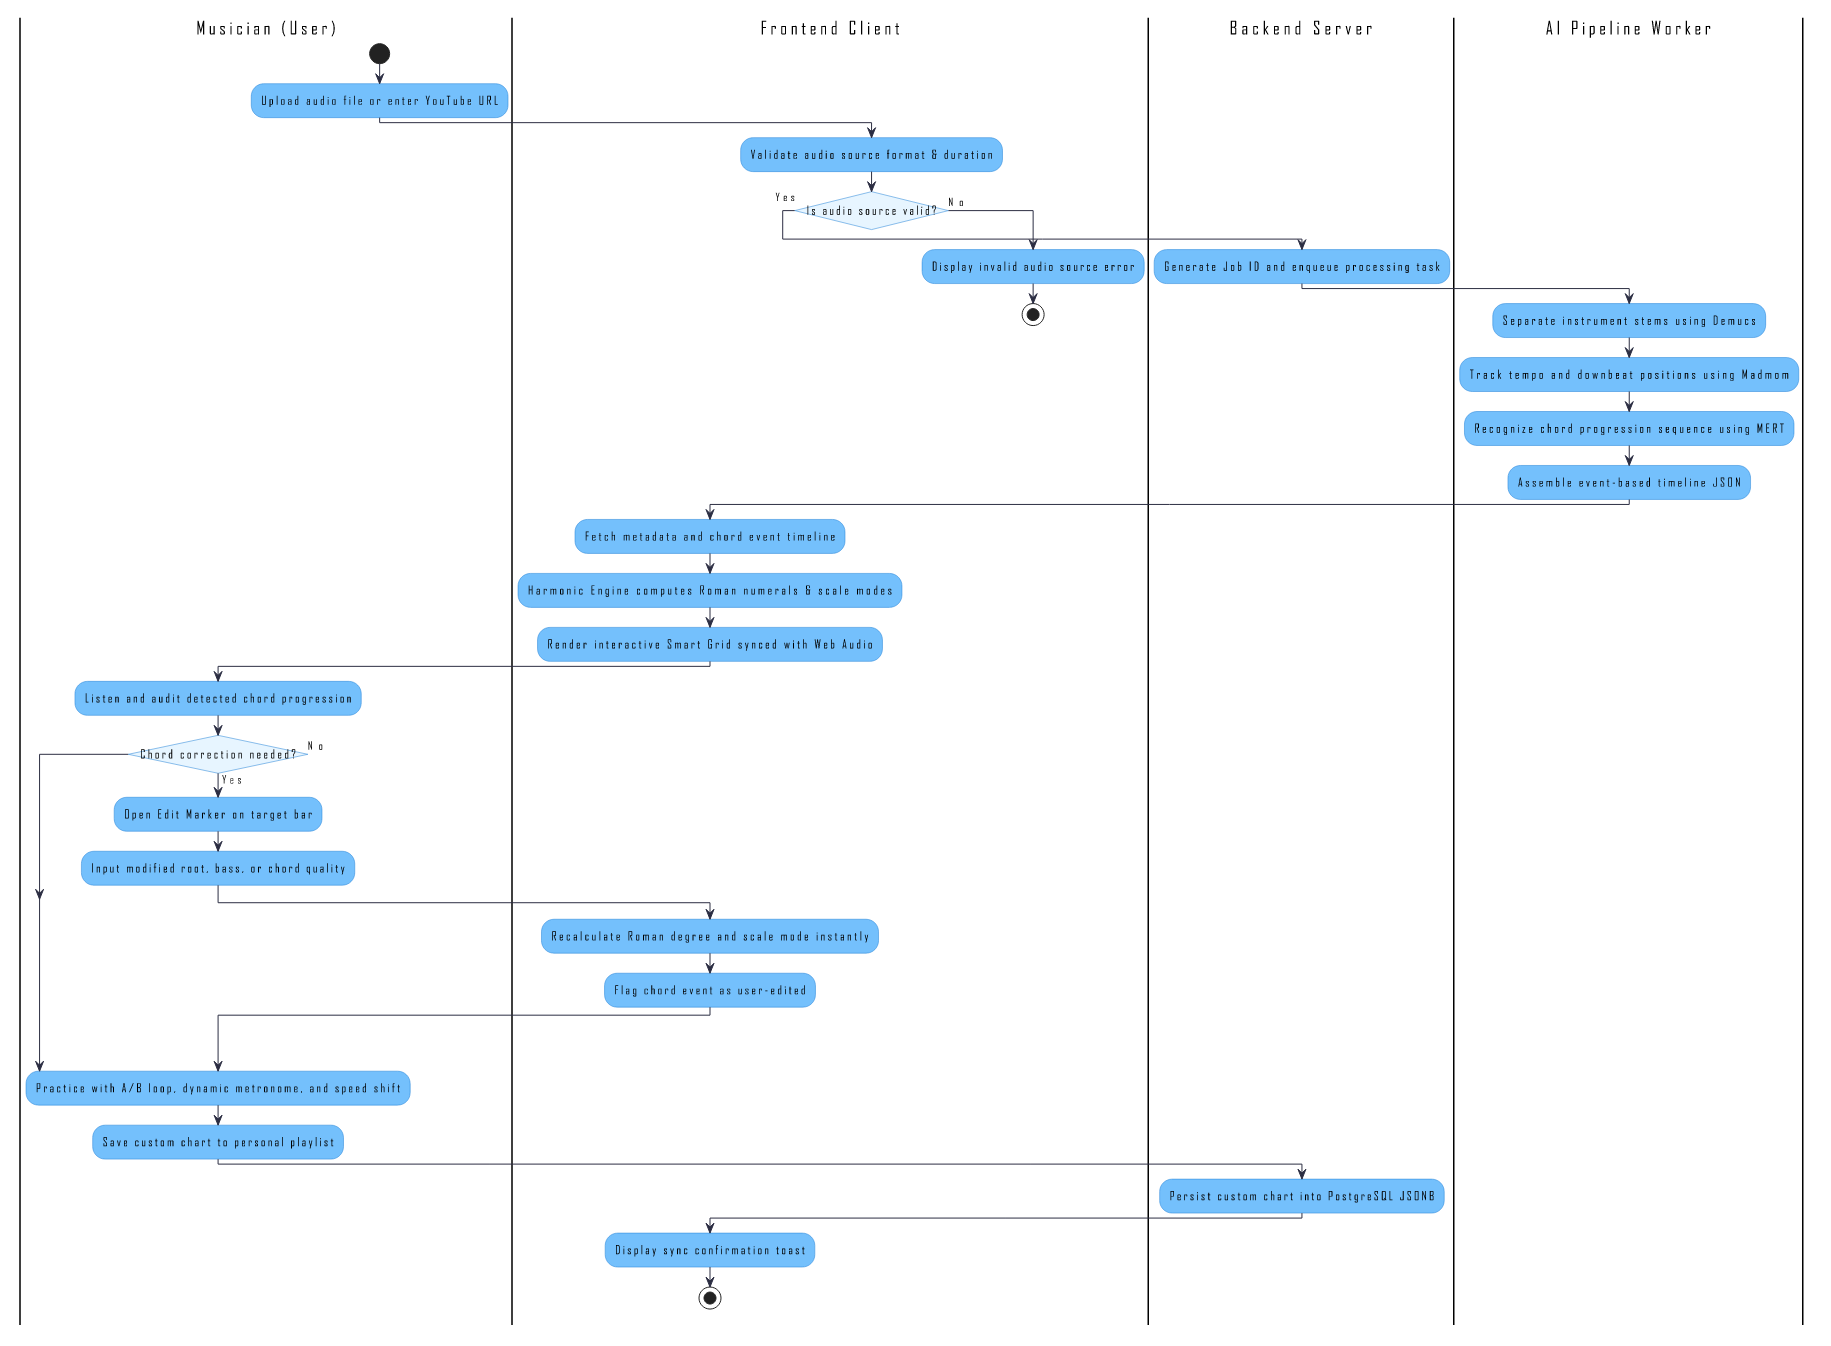
\includegraphics[width=0.95\textwidth]{activity_diagram.png}
    \caption{Activity Diagram --- ChordSense Pro Learning Flow and Practice Workspace}
    \label{fig:activity-diagram}
\end{figure}

\subsubsection{Interaction Modeling --- Use Case Diagram}

The system defines six core use cases organized around two AI interaction models:
\begin{itemize}
    \item \textbf{Human-on-the-Loop (HOTL):} The AI pipeline runs fully automatically. The user reviews and optionally corrects the output after the fact (Learning Flow, A/B Loop, Admin monitoring).
    \item \textbf{Human-in-the-Loop (HITL):} The user actively responds to AI feedback in real time during every iteration (Real-Time Practice Mode).
\end{itemize}

\begin{figure}[H]
    \centering
    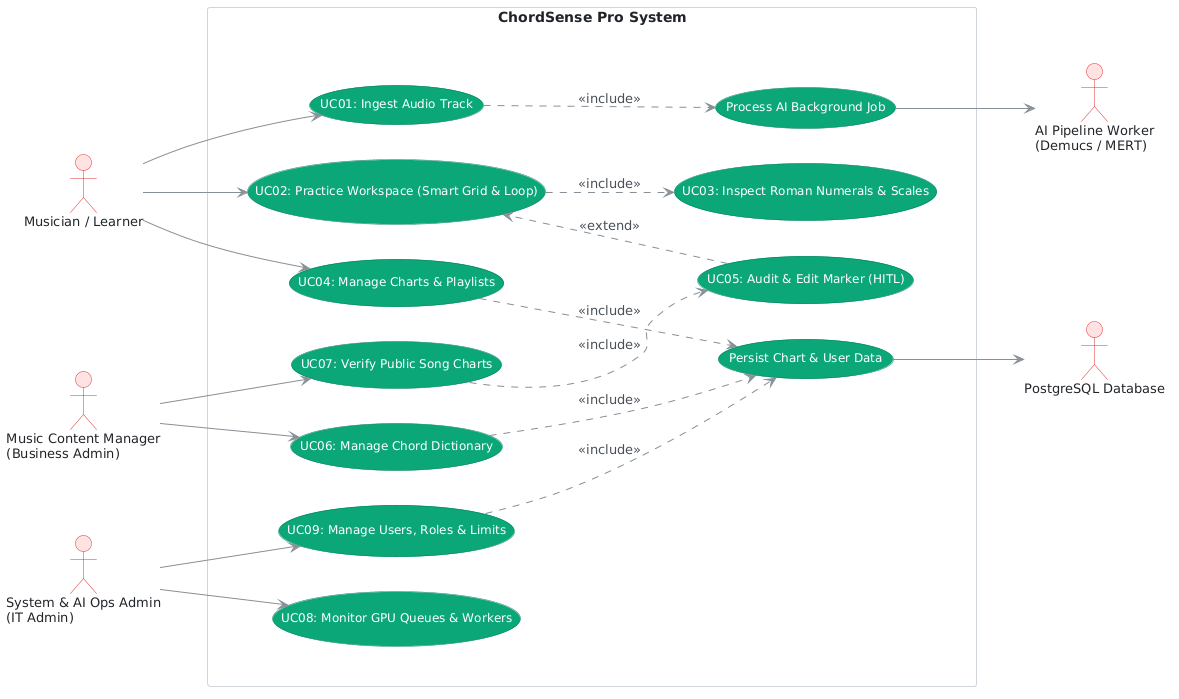
\includegraphics[width=0.92\textwidth]{usecase_diagram.png}
    \caption{Use Case Diagram --- ChordSense Pro Platform}
    \label{fig:usecase-diagram}
\end{figure}

% ─── UC table settings ────────────────────────────────────────────────
\setlength{\tabcolsep}{5pt}
\renewcommand{\arraystretch}{1.15}
\setlength{\ucLeft}{28mm}

\vspace{0.5em}
\noindent\textbf{1/ UC-01: Import and Analyze Music}

\begin{longtable}{|>{\bfseries}p{\ucLeft}|p{\dimexpr\linewidth-\ucLeft-2\tabcolsep-2\arrayrulewidth}|}
\hline
Name & Import and Analyze Music \\ \hline
ID & UC-01 \\ \hline
Actor & Primary: Musician / Learner \\ \hline
Description & User imports a song via YouTube URL or audio upload. The system dispatches the analysis job. Upon completion, the Smart Grid and harmonic annotations are displayed automatically (HOTL). \\ \hline
Preconditions &
\begin{itemize}[leftmargin=1em, nosep, topsep=2pt, partopsep=0pt, parsep=0pt, after=\strut]
    \item User is logged in
    \item YouTube URL is valid or audio file is $\leq 50\,\text{MB}$
\end{itemize}
\\ \hline
Postconditions &
\begin{itemize}[leftmargin=1em, nosep, topsep=2pt, partopsep=0pt, parsep=0pt, after=\strut]
    \item \textbf{Success:} Smart Grid rendered with chord events, Roman numeral annotations, and scale suggestions. Song saved to user library.
    \item \textbf{Failure:} Error message displayed; no data saved.
\end{itemize}
\\ \hline
Basic Flow &
\begin{enumerate}[leftmargin=1.5em, nosep, topsep=2pt, partopsep=0pt, parsep=0pt, after=\strut]
    \item User enters YouTube URL or uploads audio file
    \item System validates input and dispatches analysis job to AI Processing Service queue
    \item AI pipeline executes: yt-dlp $\rightarrow$ Demucs $\rightarrow$ madmom $\rightarrow$ MERT inference
    \item Job completion triggers frontend update via WebSocket notification
    \item Frontend renders Smart Grid with chord events and Harmonic Engine annotations
    \item Song automatically saved to user's library
\end{enumerate}
\\ \hline
Alternative Flow &
\textbf{AF1: YouTube URL is unavailable}
\begin{enumerate}[leftmargin=1.5em, nosep, topsep=2pt, partopsep=0pt, parsep=0pt, after=\strut]
    \item yt-dlp returns download error
    \item System notifies user; suggests uploading audio file directly
\end{enumerate}
\\ \hline
Exception Flow &
\textbf{EF1: AI service timeout (at step 3)}
\begin{enumerate}[leftmargin=1.5em, nosep, topsep=2pt, partopsep=0pt, parsep=0pt, after=\strut]
    \item Analysis job exceeds 60 seconds without completion
    \item System returns timeout error; user may retry or contact support
\end{enumerate}
\\ \hline
\caption{UC\_01: Import and Analyze Music}\label{tab:uc01}
\end{longtable}

\vspace{0.5em}
\noindent\textbf{2/ UC-02: A/B Loop and Practice Tools}

\begin{longtable}{|>{\bfseries}p{\ucLeft}|p{\dimexpr\linewidth-\ucLeft-2\tabcolsep-2\arrayrulewidth}|}
\hline
Name & A/B Loop and Practice Tools \\ \hline
ID & UC-02 \\ \hline
Actor & Primary: Musician / Learner \\ \hline
Description & User selects a passage in the Smart Grid for A/B loop practice with metronome and speed shift control. \\ \hline
Preconditions &
\begin{itemize}[leftmargin=1em, nosep, topsep=2pt, partopsep=0pt, parsep=0pt, after=\strut]
    \item User is logged in
    \item A song with a chord analysis result is loaded in the workspace
\end{itemize}
\\ \hline
Postconditions &
\begin{itemize}[leftmargin=1em, nosep, topsep=2pt, partopsep=0pt, parsep=0pt, after=\strut]
    \item \textbf{Success:} Selected passage loops continuously at the configured speed with metronome enabled.
\end{itemize}
\\ \hline
Basic Flow &
\begin{enumerate}[leftmargin=1.5em, nosep, topsep=2pt, partopsep=0pt, parsep=0pt, after=\strut]
    \item User drag-selects a range of bars in the Smart Grid
    \item System activates A/B Loop mode with the selected range highlighted
    \item User optionally enables the metronome (synchronized to detected song BPM)
    \item User optionally adjusts playback speed ($0.5\times$, $0.75\times$, $1.0\times$)
    \item Web Audio API begins looping the selected passage at the configured speed with pitch preserved
    \item User clicks any chord in the loop to open the Chord Dictionary
\end{enumerate}
\\ \hline
\caption{UC\_02: A/B Loop and Practice Tools}\label{tab:uc02}
\end{longtable}

\vspace{0.5em}
\noindent\textbf{3/ UC-03: Edit Marker --- Override AI Chord}

\begin{longtable}{|>{\bfseries}p{\ucLeft}|p{\dimexpr\linewidth-\ucLeft-2\tabcolsep-2\arrayrulewidth}|}
\hline
Name & Edit Marker --- Override AI Chord \\ \hline
ID & UC-03 \\ \hline
Actor & Primary: Musician / Learner; Secondary: Music Platform Manager \\ \hline
Description & User corrects an AI-detected chord label via the Edit Marker. The Harmonic Engine immediately recalculates Roman numeral and scale annotations for the updated chord. \\ \hline
Preconditions &
\begin{itemize}[leftmargin=1em, nosep, topsep=2pt, partopsep=0pt, parsep=0pt, after=\strut]
    \item User is logged in
    \item A song analysis is loaded in the workspace
\end{itemize}
\\ \hline
Postconditions &
\begin{itemize}[leftmargin=1em, nosep, topsep=2pt, partopsep=0pt, parsep=0pt, after=\strut]
    \item \textbf{Success:} Chord label updated; \texttt{is\_user\_edited = true}; Harmonic Engine recalculated; change persisted to database.
\end{itemize}
\\ \hline
Basic Flow &
\begin{enumerate}[leftmargin=1.5em, nosep, topsep=2pt, partopsep=0pt, parsep=0pt, after=\strut]
    \item User clicks a chord cell in the Smart Grid
    \item System opens Edit Marker modal showing current Root, Quality, Extension
    \item User modifies values via dropdown selectors
    \item System validates the chord combination
    \item System updates chord event in local state and sets \texttt{is\_user\_edited = true}
    \item Client-Side Harmonic Engine recalculates Roman numeral and scale for the updated chord
    \item Updated annotations displayed instantly in the Smart Grid
    \item System persists the edit to the database asynchronously
\end{enumerate}
\\ \hline
Alternative Flow &
\textbf{AF1: User resets to original AI output}
\begin{enumerate}[leftmargin=1.5em, nosep, topsep=2pt, partopsep=0pt, parsep=0pt, after=\strut]
    \item User clicks ``Reset to AI'' in the Edit Marker modal
    \item System restores AI-detected chord; \texttt{is\_user\_edited} flag cleared
    \item Harmonic Engine recalculates for the restored chord
\end{enumerate}
\\ \hline
\caption{UC\_03: Edit Marker --- Override AI Chord}\label{tab:uc03}
\end{longtable}

\vspace{0.5em}
\noindent\textbf{4/ UC-04: Real-Time Practice Mode}

\begin{longtable}{|>{\bfseries}p{\ucLeft}|p{\dimexpr\linewidth-\ucLeft-2\tabcolsep-2\arrayrulewidth}|}
\hline
Name & Real-Time Practice Mode \\ \hline
ID & UC-04 \\ \hline
Actor & Primary: Musician / Learner \\ \hline
Description & User plays an instrument in front of a microphone. The system performs real-time chord inference and provides visual feedback comparing the live chord to the target chord at the current playback position (HITL). \\ \hline
Basic Flow &
\begin{enumerate}[leftmargin=1.5em, nosep, topsep=2pt, partopsep=0pt, parsep=0pt, after=\strut]
    \item User opens Real-Time Practice tab
    \item System requests microphone access and initializes Web Audio API input stream
    \item System begins real-time chord inference on live audio ($< 200\,\text{ms}$ latency per frame)
    \item Smart Grid plays the song; at each beat, the target chord is highlighted
    \item System compares recognized live chord to target chord
    \item Correct match: cell highlighted green; incorrect: highlighted red with expected chord shown
    \item User adjusts playing technique in response to visual feedback
    \item At session end, accuracy summary and chord correctness log saved to user profile
\end{enumerate}
\\ \hline
\caption{UC\_04: Real-Time Practice Mode}\label{tab:uc04}
\end{longtable}

\vspace{0.5em}
\noindent\textbf{5/ UC-05: Music Platform Manager --- AI Quality Monitoring}

\begin{longtable}{|>{\bfseries}p{\ucLeft}|p{\dimexpr\linewidth-\ucLeft-2\tabcolsep-2\arrayrulewidth}|}
\hline
Name & Music Platform Manager --- AI Quality Monitoring \\ \hline
ID & UC-05 \\ \hline
Actor & Primary: Music Platform Manager (Business Admin) \\ \hline
Description & The Music Platform Manager monitors AI chord recognition quality KPIs on the Admin Dashboard and flags underperforming chord classes for model re-evaluation. \\ \hline
Basic Flow &
\begin{enumerate}[leftmargin=1.5em, nosep, topsep=2pt, partopsep=0pt, parsep=0pt, after=\strut]
    \item Manager navigates to Admin Dashboard $\rightarrow$ AI Quality tab
    \item System displays: accuracy by chord class, confidence histogram, user correction rate, active model version
    \item Manager reviews chord classes below the 75\% accuracy threshold
    \item Manager submits a re-evaluation request for flagged classes
    \item System notifies the Platform System Administrator via dashboard alert
\end{enumerate}
\\ \hline
\caption{UC\_05: Music Platform Manager --- AI Quality Monitoring}\label{tab:uc05}
\end{longtable}

\vspace{0.5em}
\noindent\textbf{6/ UC-06: Platform System Administrator --- Model Deployment}

\begin{longtable}{|>{\bfseries}p{\ucLeft}|p{\dimexpr\linewidth-\ucLeft-2\tabcolsep-2\arrayrulewidth}|}
\hline
Name & Platform System Administrator --- Model Deployment \\ \hline
ID & UC-06 \\ \hline
Actor & Primary: Platform System Administrator (IT Admin) \\ \hline
Description & The Platform System Administrator deploys a new LoRA adapter version and monitors system health metrics during and after rollout. \\ \hline
Basic Flow &
\begin{enumerate}[leftmargin=1.5em, nosep, topsep=2pt, partopsep=0pt, parsep=0pt, after=\strut]
    \item Admin navigates to Model Registry in IT Admin Dashboard
    \item Admin selects the new LoRA adapter version and reviews benchmark metrics
    \item Admin initiates deployment; system performs blue-green switch
    \item Admin monitors inference latency, error rate, and GPU utilization during rollout
    \item If all metrics are within thresholds, deployment is confirmed as stable
\end{enumerate}
\\ \hline
Alternative Flow &
\textbf{AF1: Performance regression detected}
\begin{enumerate}[leftmargin=1.5em, nosep, topsep=2pt, partopsep=0pt, parsep=0pt, after=\strut]
    \item Inference error rate exceeds threshold during rollout
    \item Admin triggers rollback to previous adapter version
    \item System logs deployment failure with full diagnostic report
\end{enumerate}
\\ \hline
\caption{UC\_06: Platform System Administrator --- Model Deployment}\label{tab:uc06}
\end{longtable}

\subsection{Technology Solution}

\subsubsection{Front End}

The front end is built with \textbf{React.js} (Vite build toolchain) for the following reasons:
\begin{itemize}
    \item React's component model maps naturally to the Smart Grid (each bar is a component), the Chord Dictionary modal, and the Edit Marker overlay.
    \item The \textbf{Web Audio API} --- available in all modern browsers --- provides sample-accurate scheduling for the metronome click track and pitch-preserving speed shift via \texttt{AudioContext.playbackRate} with formant correction.
    \item \texttt{requestAnimationFrame} allows the Smart Grid highlight to track audio playback position with sub-100\,ms visual precision without blocking the main thread.
    \item Client-side computation of Roman numerals and scale suggestions in the Harmonic Engine requires no server round-trip, giving instant feedback on Edit Marker changes.
\end{itemize}

\subsubsection{Back End}

The back end is built with \textbf{Python FastAPI} for the following reasons:
\begin{itemize}
    \item Native Python integration with the AI inference service (PyTorch, HuggingFace) eliminates cross-language serialization overhead.
    \item FastAPI's ASGI model supports asynchronous WebSocket connections for real-time job completion notifications.
    \item Direct \texttt{psycopg2-binary} SQL queries (without an ORM) give precise control over JSONB array operations on chord timeline data.
\end{itemize}

\subsection{System Design}

\subsubsection{Overall System Architecture}

\begin{figure}[H]
    \centering
    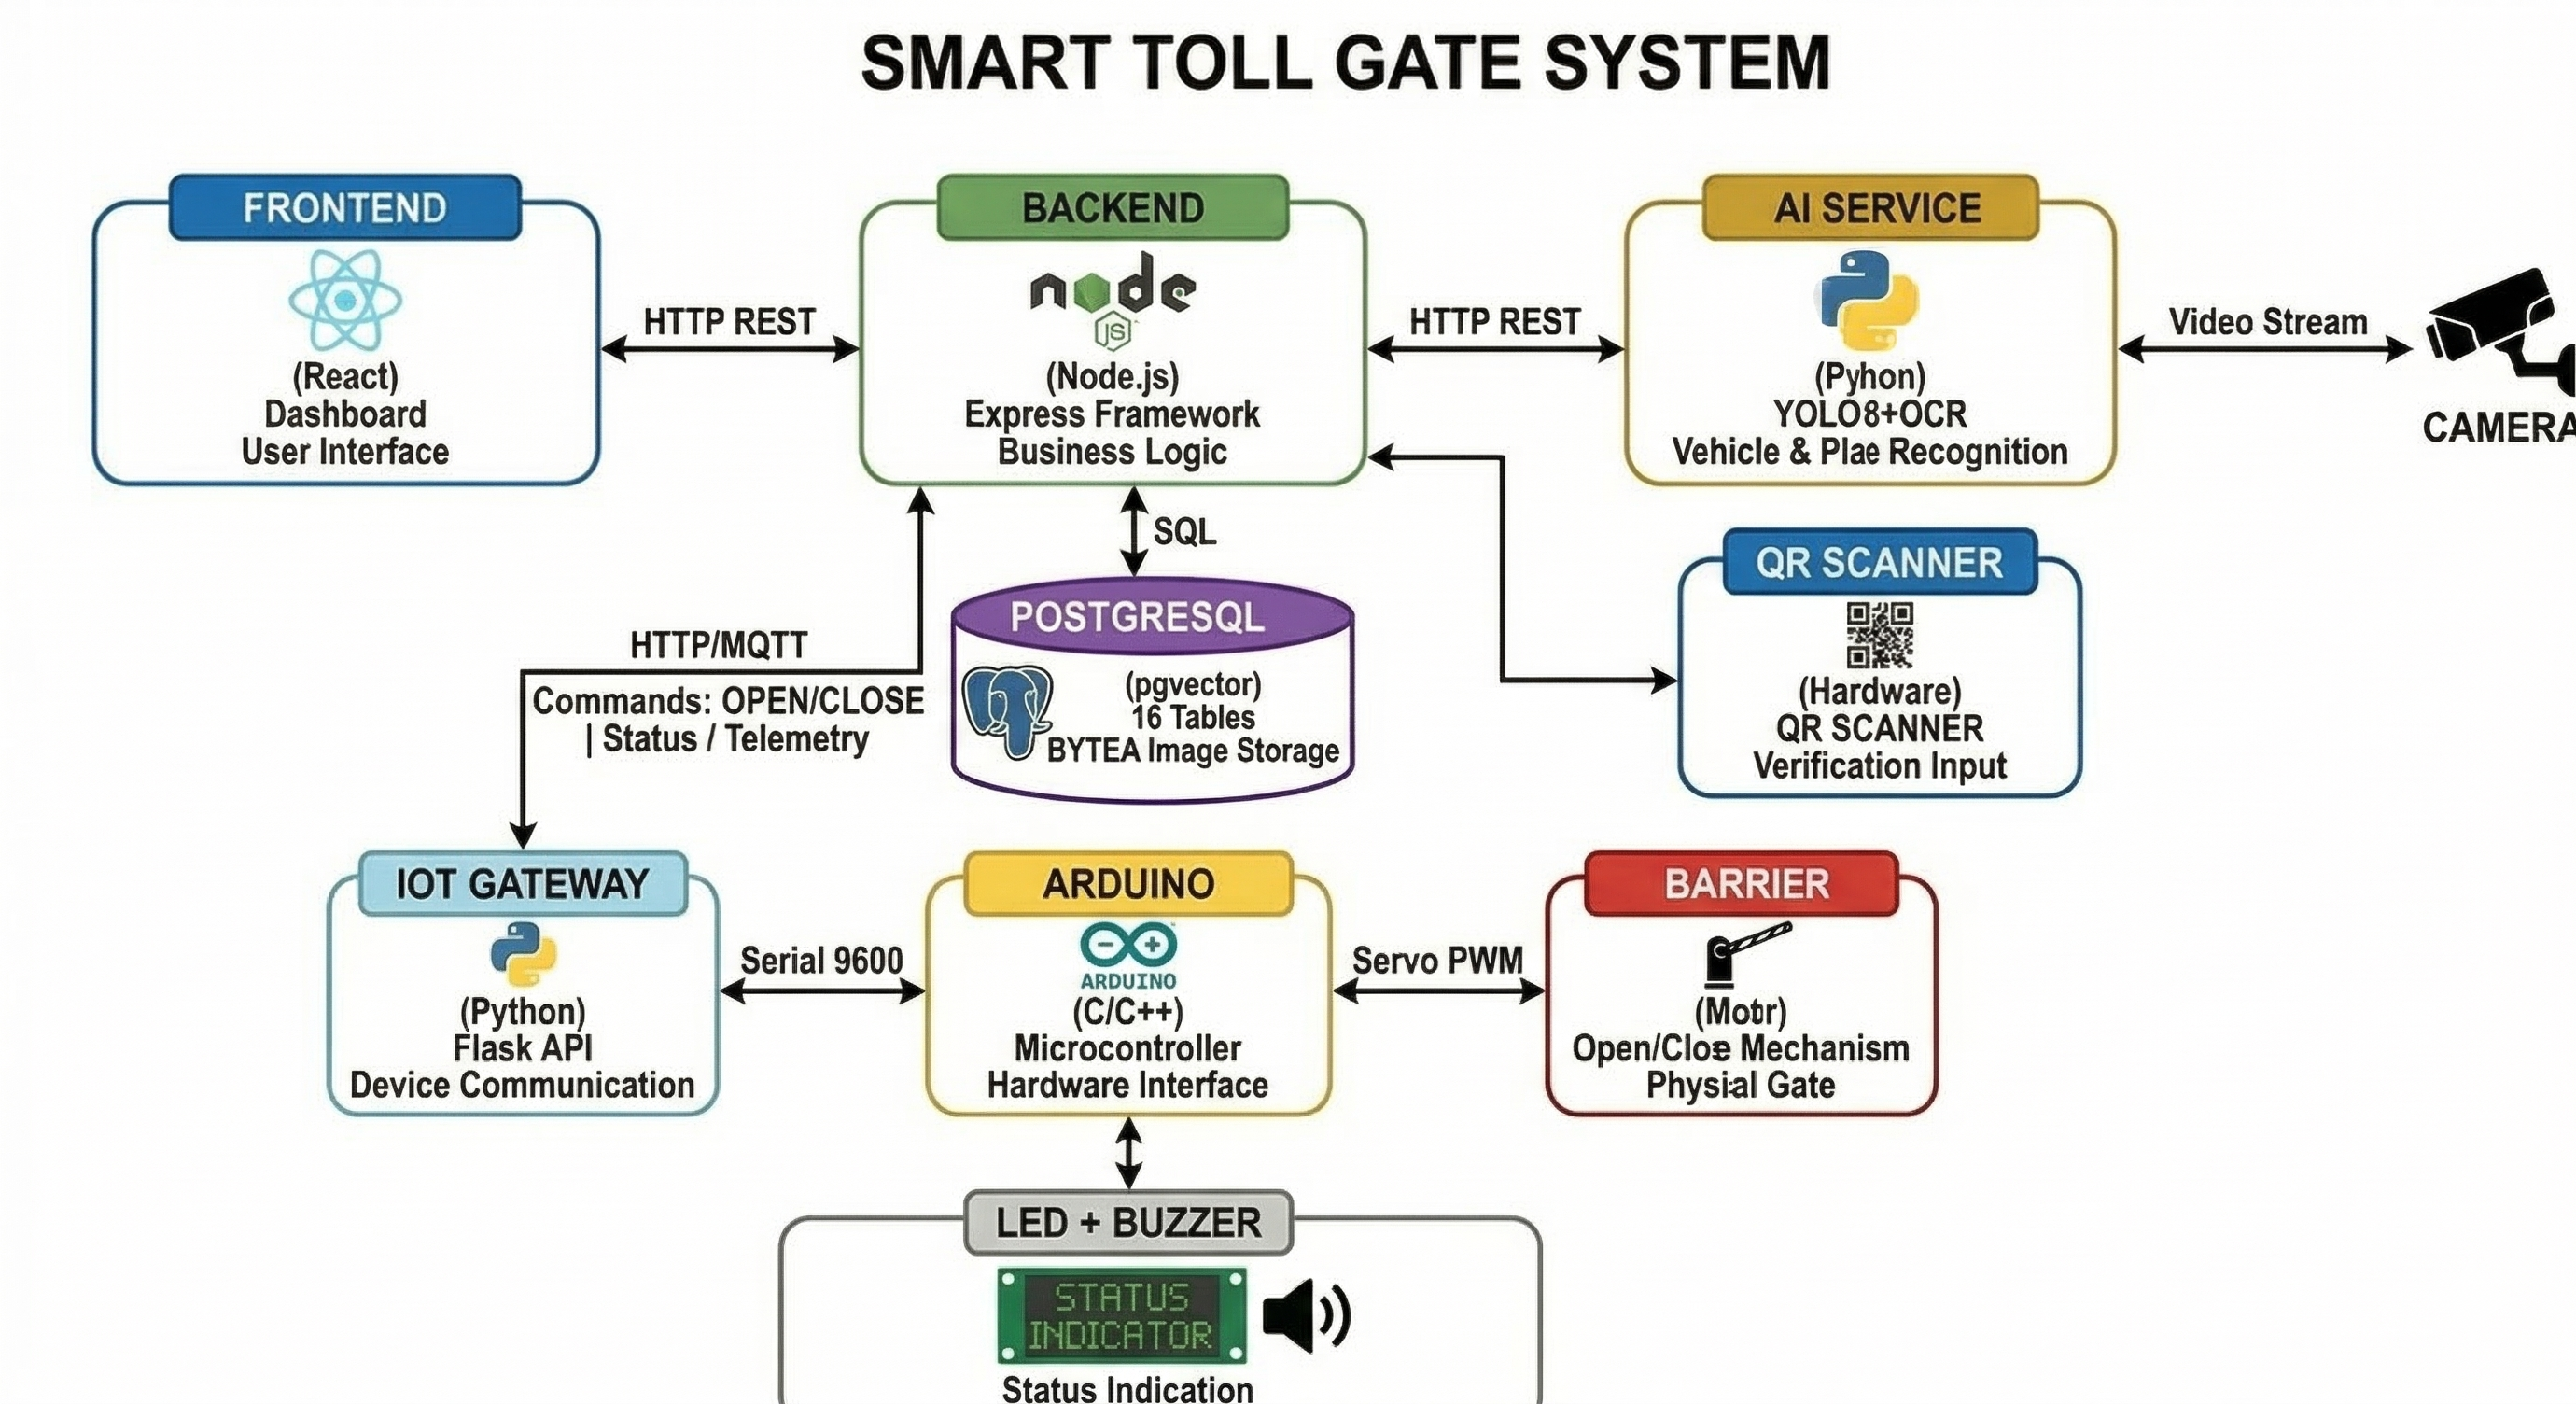
\includegraphics[width=0.95\textwidth]{overall_architecture.png}
    \caption{Overall Multi-Tier System Architecture --- ChordSense Pro}
    \label{fig:architecture}
\end{figure}

\subsubsection{Sequence Diagram}

The Sequence Diagram in Figure~\ref{fig:sequence-diagram} shows the message flow between the user, the React SPA, the FastAPI gateway, the Airflow / MongoDB data pipeline, the AI Inference Service, and PostgreSQL during a complete song analysis request.

\begin{figure}[H]
    \centering
    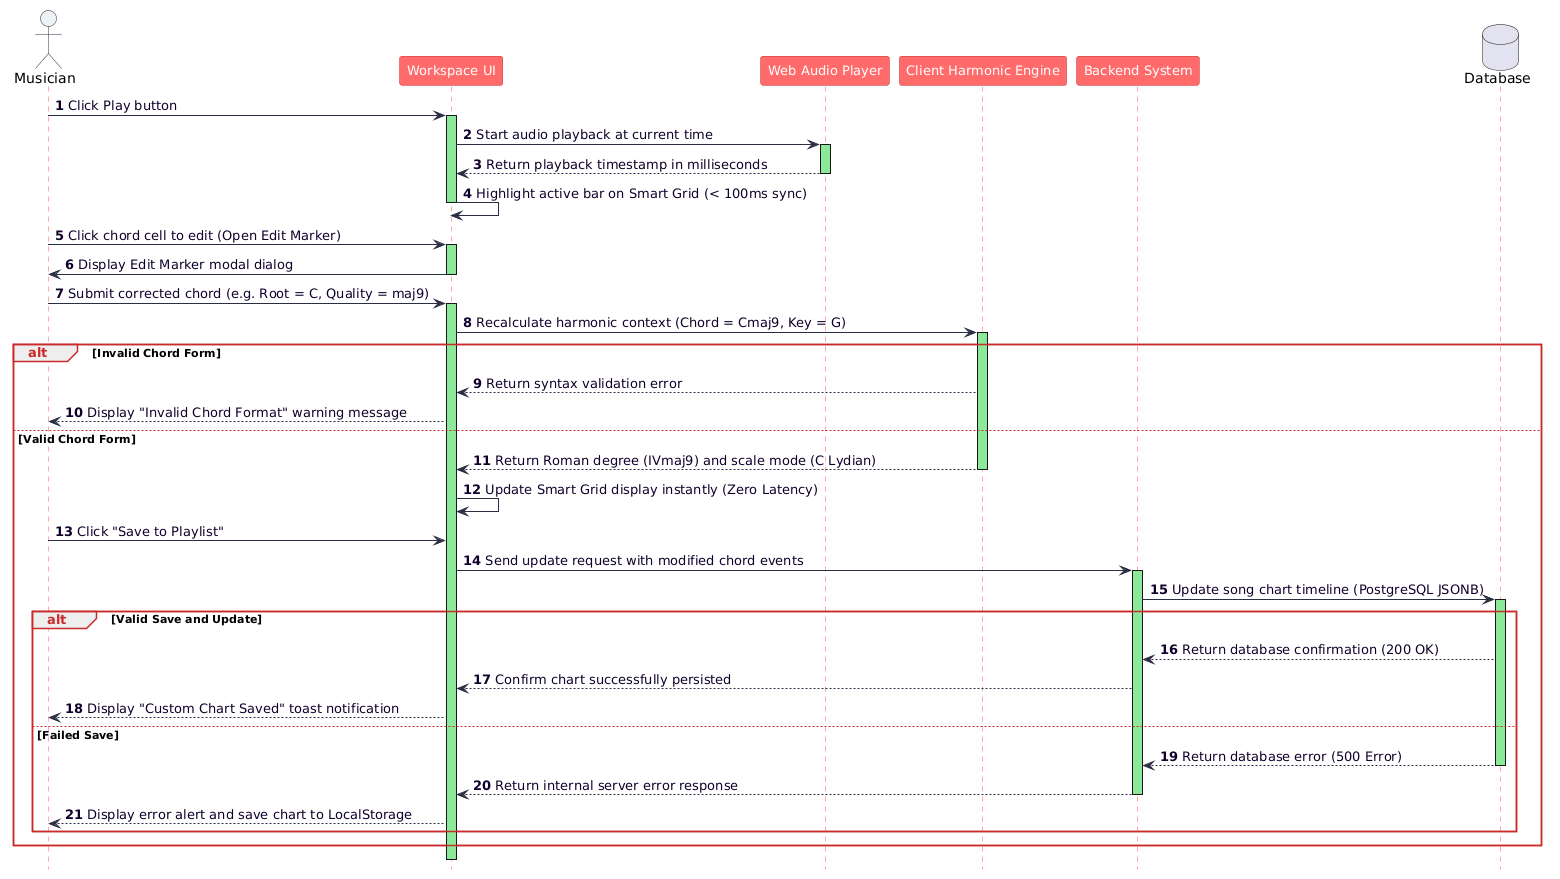
\includegraphics[width=0.95\textwidth]{sequence_diagram.png}
    \caption{Sequence Diagram --- Audio Analysis and Real-Time Interactive Workspace Execution}
    \label{fig:sequence-diagram}
\end{figure}

\subsubsection{Class Diagram}

\begin{figure}[H]
    \centering
    \includegraphics[width=0.95\textwidth]{class_diagram.png}
    \caption{Class Diagram --- Core Domain Models}
    \label{fig:class-diagram}
\end{figure}

\subsubsection{API Design}

The key REST API endpoints are listed below:

\begin{itemize}
    \item \texttt{POST /api/v1/analyze/url} --- Accept a YouTube URL; dispatch analysis job; return job ID.
    \item \texttt{POST /api/v1/analyze/file} --- Accept an uploaded audio file; dispatch analysis job; return job ID.
    \item \texttt{GET /api/v1/analyze/status/\{id\}} --- Poll analysis job status (queued, processing, done, failed).
    \item \texttt{GET /api/v1/charts/\{id\}} --- Retrieve full JSONB chord event timeline and metadata for rendering the Smart Grid.
    \item \texttt{PATCH /api/v1/charts/\{id\}/events} --- Submit user chord edits; marks modified events with \texttt{is\_user\_edited = true}.
    \item \texttt{POST /api/v1/playlists} --- Create a new playlist.
    \item \texttt{GET /api/v1/playlists} --- List all playlists for the authenticated user.
    \item \texttt{POST /api/v1/playlists/\{id\}/add} --- Add a song chart to a playlist.
    \item \texttt{GET /api/v1/dictionary/search?root=C\&quality=maj9} --- Query the chord dictionary for fingering data.
    \item \texttt{POST /api/v1/recognize} --- Real-time chord inference: accepts 2-second base64 WAV; returns chord label with confidence.
\end{itemize}

\subsubsection{UI/UX Design}

The user interface is organized around the \textbf{Practice Workspace}, which contains:
\begin{itemize}
    \item \textbf{Smart Grid View:} A scrollable grid where each cell represents one bar. The currently playing bar is highlighted in real time. The key and tempo are shown in the header. Roman numerals and scale names appear below each chord name.
    \item \textbf{Audio Player Bar:} Standard transport controls (play, pause, seek) plus speed toggle buttons (0.5$\times$, 0.75$\times$, 1$\times$) and a metronome toggle.
    \item \textbf{Chord Dictionary Panel:} Opens as a side drawer when the user clicks a chord cell. Displays guitar fretboard fingering diagrams, piano keyboard diagrams, and a play button that triggers the Soundfont synthesizer.
    \item \textbf{Edit Marker Modal:} Opens on long-press or right-click of a chord cell. Provides dropdowns for Root, Quality, and Extension. Changes update the Smart Grid and Harmonic Engine annotations instantly.
    \item \textbf{Basic/Precise Toggle:} A switch in the top toolbar. In Basic mode, extended chord suffixes are stripped client-side (G9sus4 $\to$ G) for readability. Switching is instant with no API call.
\end{itemize}

\subsubsection{Third-Party Policies and Data Handling}

\begin{itemize}
    \item \textbf{YouTube audio download:} Audio is downloaded using yt-dlp under the YouTube Terms of Service fair-use provision for personal, non-commercial music analysis. The downloaded audio is processed server-side and not redistributed.
    \item \textbf{User audio data:} Microphone audio captured during Real-Time Practice Mode is processed in-memory for chord inference. A short 2-second audio clip is optionally stored in MongoDB with a 30-day TTL for model improvement, subject to user consent.
    \item \textbf{Authentication:} JWT tokens with configurable expiry are used. Passwords are hashed with bcrypt before storage.
\end{itemize}

\subsection{Chapter Summary}

This chapter covered the business process model, use case specifications, technology selection rationale, and detailed system design for the Front End and Back End. The next chapter describes the Data Engineering pipeline that feeds processed audio features into the chord recognition model.

\newpage
%===========================================
% CHAPTER 6: DATA ENGINEERING PIPELINE
%===========================================
\section{Data Engineering Pipeline}

\subsection{Architecture Definition and Design Rationale}

The data engineering pipeline is organized using \textbf{Domain-Driven Design (DDD)} with the \textbf{Onion Architecture} (Figure~\ref{fig:ddd-onion}). This architecture pattern was selected over simpler alternatives for the following reasons:

\begin{figure}[H]
    \centering
    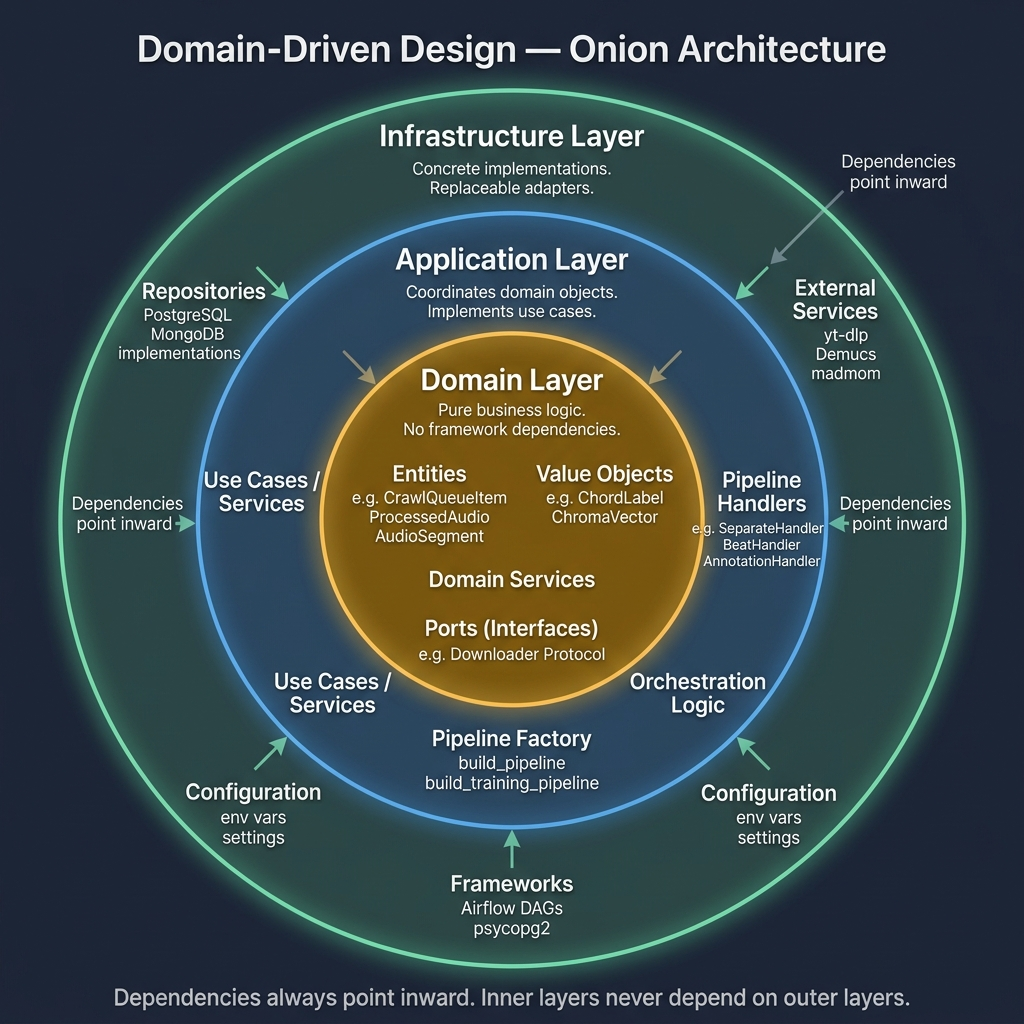
\includegraphics[width=0.6\textwidth]{image/ddd_onion_architecture.jpg}
    \caption{DDD Onion Architecture --- Domain Layer at the core, Application Layer in the middle, Infrastructure Layer at the outermost ring.}
    \label{fig:ddd-onion}
\end{figure}

\begin{longtable}{@{}
    >{\raggedright\arraybackslash}p{0.22\linewidth}
    >{\raggedright\arraybackslash}p{0.22\linewidth}
    >{\raggedright\arraybackslash}p{0.50\linewidth}@{}}

    \caption{Architecture Comparison: DDD Onion vs.\ Alternatives}\label{tab:arch_compare} \\
    \toprule
    \textbf{Architecture} & \textbf{Characteristic} & \textbf{Evaluation for This Project} \\
    \midrule
    \endfirsthead
    \multicolumn{3}{l}{\footnotesize\itshape (Table~\ref{tab:arch_compare} continued)}\\
    \toprule
    \textbf{Architecture} & \textbf{Characteristic} & \textbf{Evaluation for This Project} \\
    \midrule
    \endhead
    \bottomrule
    \endlastfoot

    Monolithic ETL script & All logic in one file & Simple but fragile: adding a new dataset source forces changes across the entire script. \\
    \addlinespace
    Layered MVC & Controller / Service / Repository & Good separation, but no concept of Bounded Contexts. Cross-domain coupling is common. \\
    \addlinespace
    \textbf{DDD Onion} (selected) & Bounded Contexts + inward dependency rule & Each data source and processing stage is isolated. Adding a new dataset only requires a new downloader adapter. Domain logic has no framework imports. \\
\end{longtable}

The key structural principle is that \textbf{dependencies always point inward}. The Domain Layer (core business entities and port interfaces) knows nothing about databases or external services. The Infrastructure Layer (concrete implementations) depends on the Domain Layer, not the other way around.

\subsection{Layer-by-Layer Implementation}

The pipeline is organized into five Bounded Contexts. Table~\ref{tab:bounded_contexts} describes each context and its responsibilities.

\begin{longtable}{@{}
    >{\raggedright\arraybackslash}p{0.22\linewidth}
    >{\raggedright\arraybackslash}p{0.22\linewidth}
    >{\raggedright\arraybackslash}p{0.50\linewidth}@{}}

    \caption{DDD Bounded Contexts and Their Responsibilities}\label{tab:bounded_contexts} \\
    \toprule
    \textbf{Bounded Context} & \textbf{Package} & \textbf{Responsibility} \\
    \midrule
    \endfirsthead
    \multicolumn{3}{l}{\footnotesize\itshape (Table~\ref{tab:bounded_contexts} continued)}\\
    \toprule
    \textbf{Bounded Context} & \textbf{Package} & \textbf{Responsibility} \\
    \midrule
    \endhead
    \bottomrule
    \endlastfoot

    Shared Kernel & \texttt{src/shared/} & Base entity class, value objects (\texttt{ChordLabel}, \texttt{ChromaVector}), database connection pools, and environment-based configuration. \\
    \addlinespace
    Orchestration & \texttt{src/data\_ingest/} & Manages the crawl queue state machine (\texttt{pending}$\to$\texttt{running}$\to$\texttt{done}/\texttt{failed}), coordinates download dispatch, and bridges DAG~1 output to DAG~2 input via MongoDB staging. \\
    \addlinespace
    Audio Acquisition & \texttt{src/data\_loader/} & Defines the \texttt{Downloader} port and provides seven concrete adapters (JAAH, ChoCo, McGill, RWC, Kaggle, Pianoteq, Local). An \texttt{AudioDispatcher} registry maps \texttt{AudioSource} enum values to the correct downloader at runtime (Strategy pattern). \\
    \addlinespace
    Audio Transform & \texttt{src/data\_processing/} & Implements the processing handler chain: source separation, beat tracking, segmentation, annotation parsing, chord summarization, data augmentation, and feature extraction. Uses the Chain of Responsibility pattern. \\
    \addlinespace
    Analysis Output & \texttt{src/song\_analysis/} & Persists the final \texttt{SongAnalysis} aggregate (detected key, chord timeline, chord sheet) into PostgreSQL for downstream consumption by the web application. \\
    \addlinespace
    Student Analytics & \texttt{src/user\_analytics/} & Stores individual chord practice attempts and computes rolling mastery metrics per student per chord (daily aggregation by DAG~3). \\
\end{longtable}

\subsubsection{Audio Acquisition Layer (data\_loader)}

This layer defines a \texttt{Downloader} Protocol (port interface). The \texttt{AudioDispatcher} acts as a registry: at startup, each concrete downloader is registered against its corresponding \texttt{AudioSource} enum value. When a download is requested, the dispatcher looks up the correct downloader and delegates the call.

The seven concrete downloader adapters and their data sources are:
\begin{itemize}
    \item \textbf{JaahDownloader} --- JAAH dataset: 113 jazz tracks from Zenodo (direct HTTP download).
    \item \textbf{McGillDownloader} --- McGill Billboard: 1,300 pop/rock tracks via yt-dlp YouTube search.
    \item \textbf{ChocoDownloader} --- ChoCo corpus: 20,000 tracks via yt-dlp YouTube URLs.
    \item \textbf{RwcDownloader} --- RWC Popular Music: 100 Japanese pop tracks (local archive copy).
    \item \textbf{KaggleDownloader} --- Kaggle Guitar Chord Dataset v3: 7,000+ recordings via Kaggle CLI.
    \item \textbf{PianoteqDownloader} --- Synthetic piano data rendered by the Pianoteq physical modeling synthesizer.
    \item \textbf{LocalFileDownloader} --- Local files already on disk (used for manual additions and testing).
\end{itemize}

\subsubsection{Audio Transform Layer (data\_processing)}

Each processing step is implemented as a \texttt{BaseProcessingHandler} subclass. The factory method \texttt{build\_training\_pipeline()} wires all seven handlers into a chain:

\begin{center}
\texttt{Separate} $\to$ \texttt{Beat} $\to$ \texttt{Segment} $\to$ \texttt{Annotation} $\to$ \texttt{Summary} $\to$ \texttt{Augment} $\to$ \texttt{Feature}
\end{center}

For the inference pipeline (no augmentation), only five handlers are used:

\begin{center}
\texttt{Separate} $\to$ \texttt{Beat} $\to$ \texttt{Segment} $\to$ \texttt{Summary} $\to$ \texttt{Feature}
\end{center}

Table~\ref{tab:handlers} describes the input and output of each handler.

\begin{longtable}{@{}
    >{\raggedright\arraybackslash}p{0.22\linewidth}
    >{\raggedright\arraybackslash}p{0.35\linewidth}
    >{\raggedright\arraybackslash}p{0.37\linewidth}@{}}

    \caption{Pipeline Handler Chain: Input and Output}\label{tab:handlers} \\
    \toprule
    \textbf{Handler} & \textbf{Input} & \textbf{Output (added to ProcessedAudio)} \\
    \midrule
    \endfirsthead
    \multicolumn{3}{l}{\footnotesize\itshape (Table~\ref{tab:handlers} continued)}\\
    \toprule
    \textbf{Handler} & \textbf{Input} & \textbf{Output (added to ProcessedAudio)} \\
    \midrule
    \endhead
    \bottomrule
    \endlastfoot

    SeparateHandler & WAV file path & Isolated harmonic stem WAV (Demucs \texttt{htdemucs} model) \\
    \addlinespace
    BeatHandler & Harmonic stem WAV & Beat times (seconds), tempo (BPM), time signature \\
    \addlinespace
    SegmentHandler & Harmonic stem + beat times & List of 2-second audio segments aligned to beat boundaries \\
    \addlinespace
    AnnotationHandler & Segments + annotation file path & Per-segment chord labels from JAMS / JAAH / Harte / RWC CSV / Kaggle filename \\
    \addlinespace
    SummaryHandler & Segments + labels & Chord timeline (start/end/chord), detected key \\
    \addlinespace
    AugmentHandler & Segments + labels & Pitch-shifted copies ($\pm$6 semitones) + noise variants; label-aware oversampling for rare extended chords \\
    \addlinespace
    FeatureHandler & Segments (original + augmented) & Chroma CQT, Mel-spectrogram, HPSS harmonic component per segment \\
\end{longtable}

The annotation parser module supports six formats: JAMS (\texttt{JamsParser}), JAAH custom JSON (\texttt{JaahParser}), Harte notation (\texttt{HarteParser}), RWC CSV (\texttt{RwcParser}), and Kaggle filename convention. This makes the pipeline dataset-agnostic: adding a new dataset only requires adding a new parser.

\subsubsection{Orchestration Layer (data\_ingest)}

The Orchestration layer manages two services that correspond to the two ETL DAGs:
\begin{itemize}
    \item \textbf{IngestRawService (DAG 1):} Reads pending URLs from the \texttt{crawl\_queue} PostgreSQL table, calls \texttt{run\_data\_loader()} to download the WAV file, downloads any associated annotation file, and saves a \texttt{RawAudioJob} document to MongoDB. This is the Extract (E) phase.
    \item \textbf{ProcessAudioService (DAG 2):} Reads pending \texttt{RawAudioJob} documents from MongoDB, validates that the WAV file exists on disk, runs the training pipeline chain, and saves the completed \texttt{SongAnalysis} to PostgreSQL. Cleans up temporary files afterwards. This is the Transform + Load (T+L) phase.
\end{itemize}

MongoDB acts as a decoupling layer between DAG 1 and DAG 2. If a download fails, it does not block the processing of audio files that were already downloaded. DAG 2 can also be re-triggered without re-downloading any files.

\subsection{Data Flow and Pipeline Architecture}

Figure~\ref{fig:pipeline} illustrates the full three-DAG ETL architecture.

\begin{figure}[H]
    \centering
    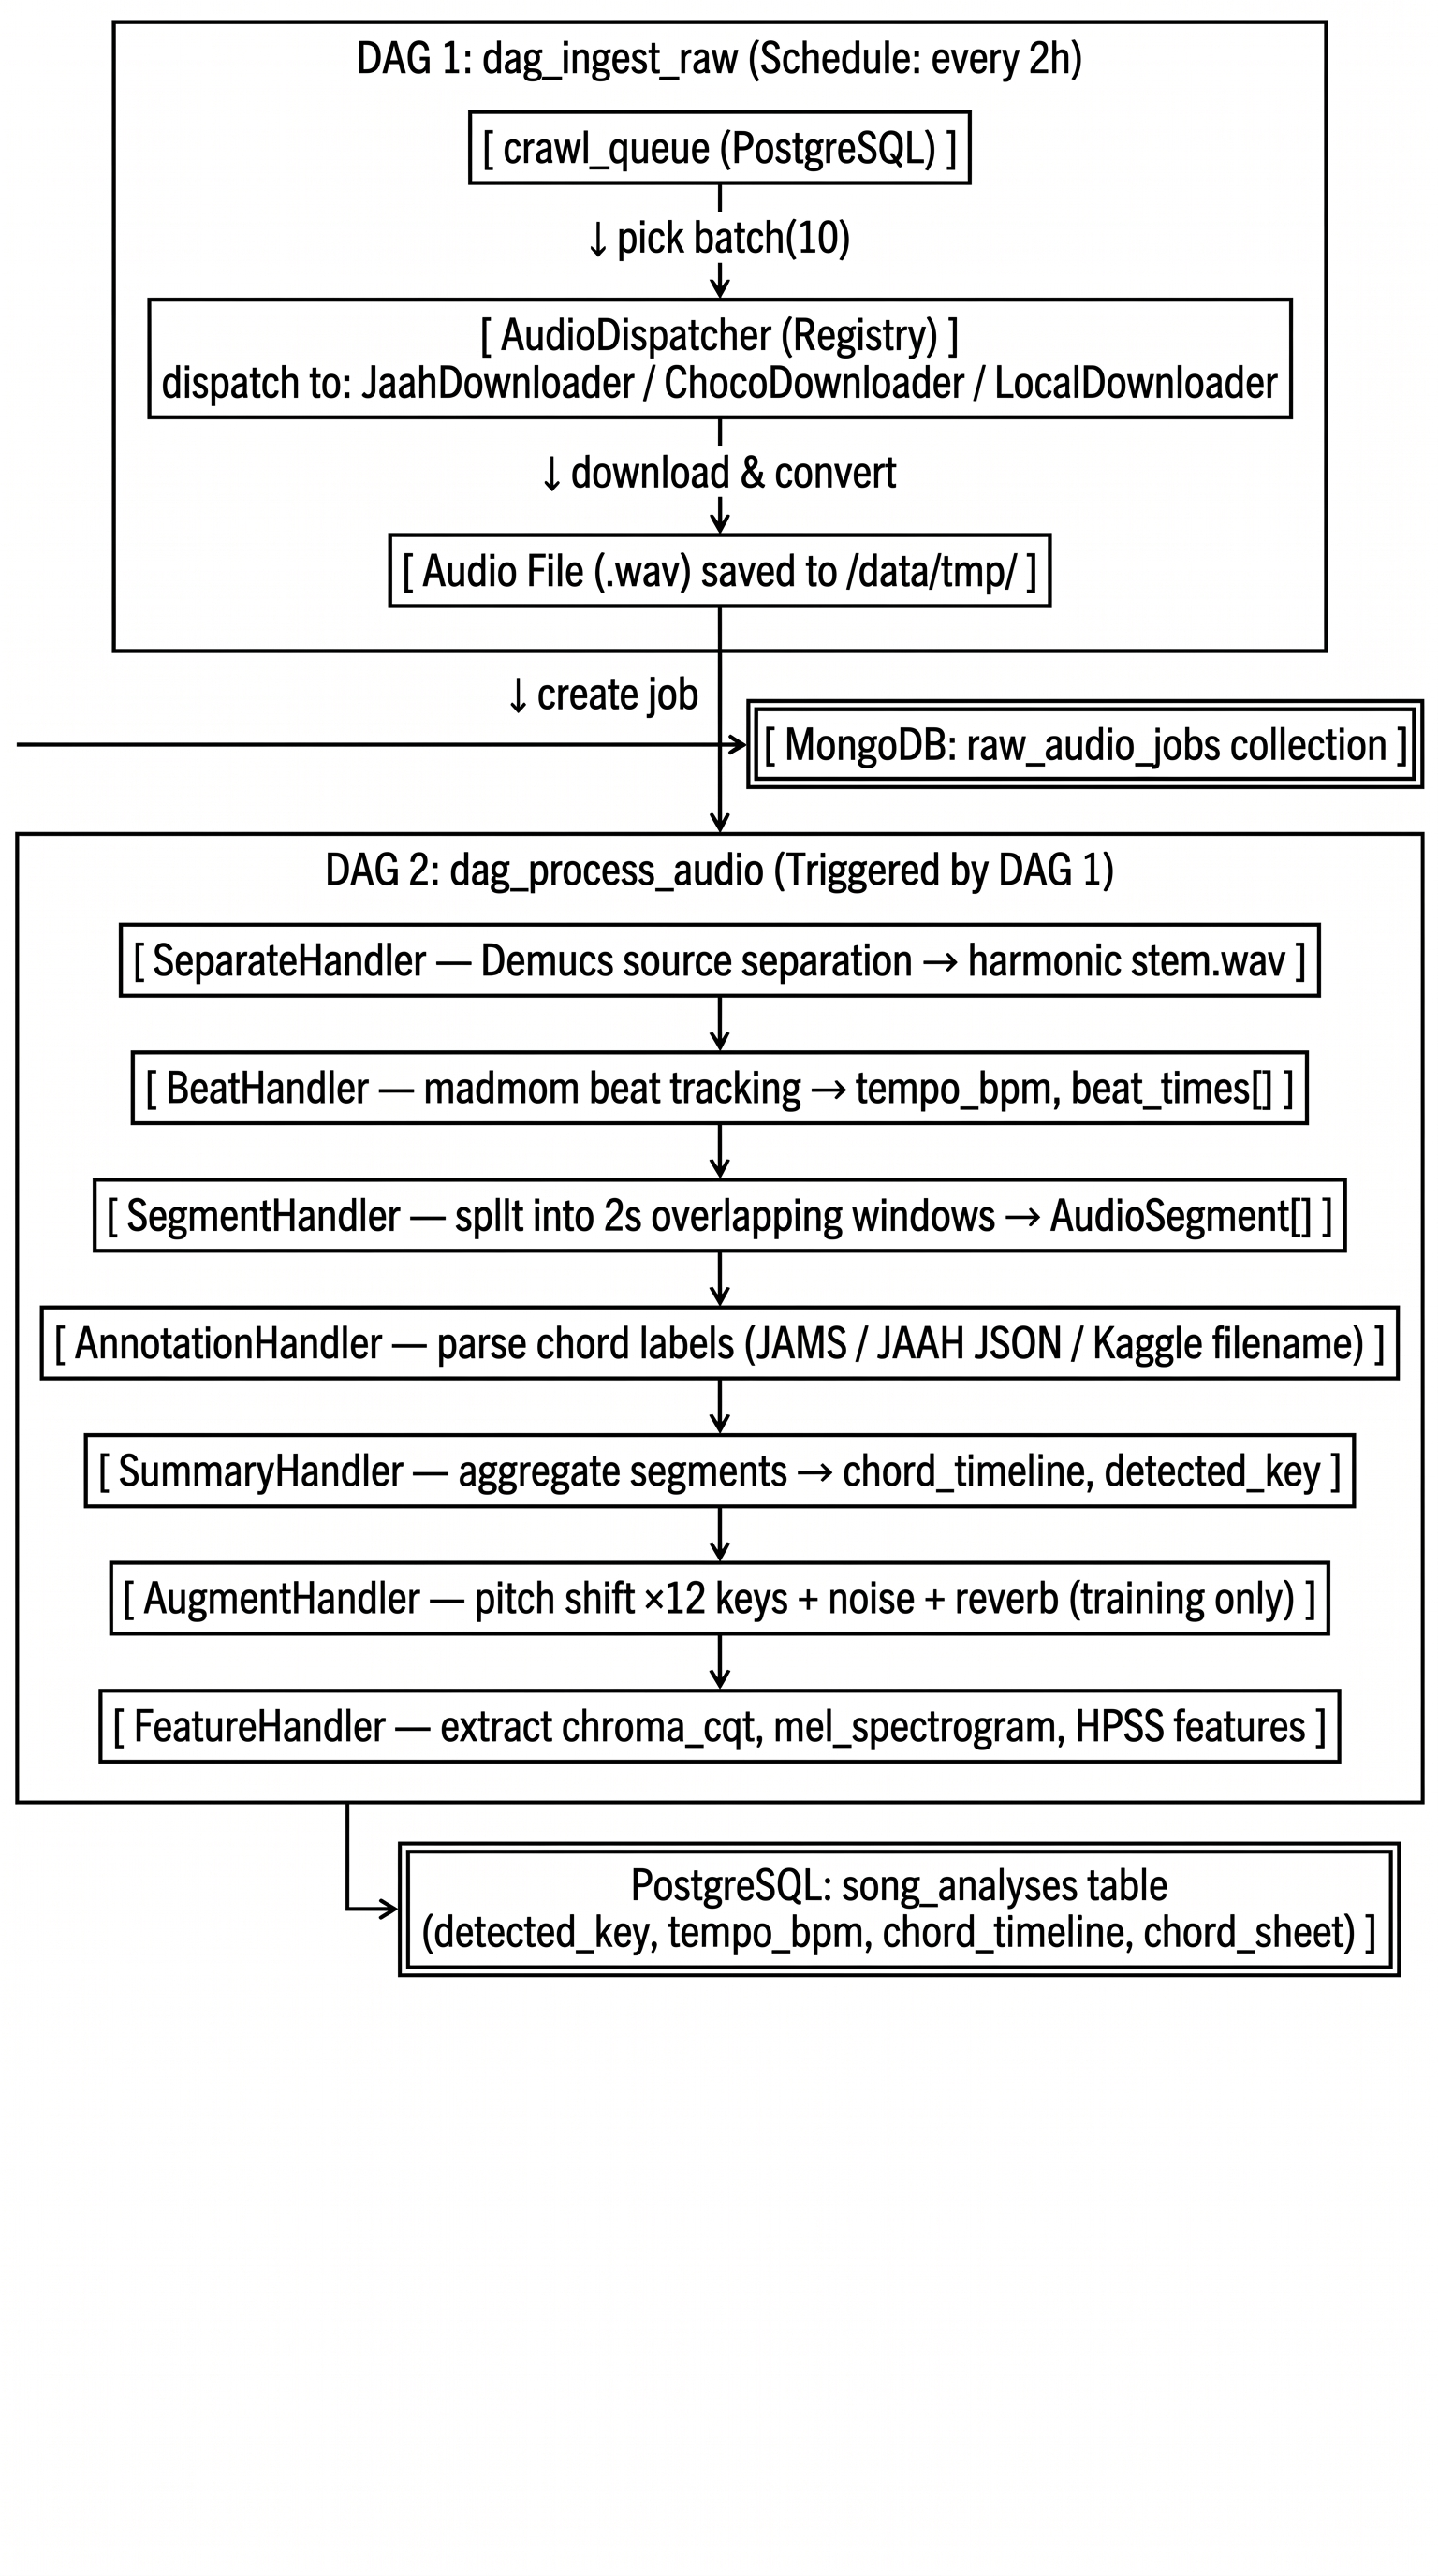
\includegraphics[width=\linewidth]{image/pipeline.jpg}
    \caption{Data Engineering Pipeline --- Three-DAG ETL Architecture with Chain of Responsibility Handler Flow}
    \label{fig:pipeline}
\end{figure}

\subsubsection{DAG 1: dag\_ingest\_raw (Extract) --- Every 2 Hours}

\begin{center}
\texttt{pick\_urls} $\to$ \texttt{download\_and\_stage} $\to$ \texttt{send\_summary} $\to$ \texttt{trigger\_dag\_process}
\end{center}

The DAG reads up to 10 pending rows from \texttt{crawl\_queue}, calls the \texttt{AudioDispatcher} to download each audio file, stages the \texttt{RawAudioJob} to MongoDB, and then fires \texttt{dag\_process\_audio} via a \texttt{TriggerDagRunOperator} (fire-and-forget, no wait).

\subsubsection{DAG 2: dag\_process\_audio (Transform + Load) --- Triggered by DAG 1}

\begin{center}
\texttt{pick\_pending\_jobs} $\to$ \texttt{process\_and\_save} $\to$ \texttt{send\_summary}
\end{center}

The DAG reads pending \texttt{RawAudioJob} documents from MongoDB and runs the full training handler chain on each one. The resulting chord timeline, detected key, and tempo are saved to the \texttt{song\_analyses} PostgreSQL table. Temporary WAV files and stems are deleted after a successful save.

\subsubsection{DAG 3: dag\_analytics\_rollup (Analytics) --- Nightly at 23:30}

\begin{center}
\texttt{aggregate\_attempts} $\to$ \texttt{rolling\_accuracy} $\to$ \texttt{update\_mastery}
\end{center}

This DAG aggregates all chord practice attempts recorded since the previous run, computes a rolling 3-day accuracy score per student per chord, and updates the \texttt{user\_chord\_mastery} table. This powers the student progress dashboard.

\subsection{Database Schema}

\subsubsection{PostgreSQL Tables}

\begin{itemize}
    \item \textbf{crawl\_queue} (id, source\_url, annotation\_url, source\_type, status, priority, error\_message, created\_at, processed\_at) --- URL queue managed by DAG 1. Status transitions: \texttt{pending} $\to$ \texttt{running} $\to$ \texttt{done} or \texttt{failed}.
    \item \textbf{song\_analyses} (id, user\_id, source\_url, song\_title, status, detected\_key, tempo\_bpm, chord\_timeline, chord\_sheet, learning\_plan, error\_message, created\_at, updated\_at) --- Final output from DAG 2. \texttt{chord\_timeline} and \texttt{chord\_sheet} are JSONB columns.
    \item \textbf{chord\_attempts} (id, user\_id, chord\_label, is\_correct, confidence, response\_time, attempted\_at) --- Individual practice attempts from Real-Time Practice Mode.
    \item \textbf{user\_chord\_mastery} (user\_id, chord\_label, mastery\_level, total\_attempts, correct\_count, last\_practiced, is\_mastered) --- Aggregated mastery per (user, chord). Updated nightly by DAG 3.
\end{itemize}

\subsubsection{MongoDB Collections}

\begin{itemize}
    \item \textbf{raw\_audio\_jobs} --- Staging queue holding job metadata, WAV file paths, and annotation paths. Acts as the bridge between DAG 1 and DAG 2.
    \item \textbf{raw\_audio} --- Binary audio clips from student practice sessions (TTL: 30 days).
    \item \textbf{mel\_spectrograms} --- Mel-spectrogram matrices ($128 \times T$) cached for rapid model retraining (TTL: 90 days).
    \item \textbf{training\_samples} --- Preprocessed training segments from academic datasets.
    \item \textbf{song\_audio\_cache} --- Post-Demucs harmonic stems cached for 7 days to avoid redundant processing.
\end{itemize}

\subsection{Technology Choice: Database Selection}

The pipeline uses two databases. Each one is chosen for a specific stage, because the two stages have very different needs.

\subsubsection{Staging Layer: Why MongoDB?}

Between DAG~1 and DAG~2, the system needs a place to temporarily hold raw audio jobs. At this point, each dataset source has a slightly different structure. Some jobs have annotation file paths, others do not. Some have YouTube URLs, others point to local files. The staging database must accept all of these without requiring a fixed schema. It also needs to handle many fast writes, and it should be able to delete old data automatically when it is no longer needed.

Table~\ref{tab:db_staging} compares three candidate databases for this role.

\begin{longtable}{@{}
    >{\raggedright\arraybackslash}p{0.27\linewidth}
    >{\raggedright\arraybackslash}p{0.22\linewidth}
    >{\raggedright\arraybackslash}p{0.22\linewidth}
    >{\raggedright\arraybackslash}p{0.22\linewidth}@{}}

    \caption{Database Comparison for the Staging Layer}\label{tab:db_staging} \\
    \toprule
    \textbf{Criterion} & \textbf{MongoDB} & \textbf{PostgreSQL} & \textbf{Cassandra} \\
    \midrule
    \endfirsthead
    \toprule
    \textbf{Criterion} & \textbf{MongoDB} & \textbf{PostgreSQL} & \textbf{Cassandra} \\
    \midrule
    \endhead
    \bottomrule
    \endlastfoot

    Schema flexibility &
    \cmark~Schema-less. Any field can be added to a document freely. &
    \xmark~Fixed schema. Every new field needs a migration script. &
    Partial. Column family must be defined upfront. \\
    \addlinespace

    Write throughput &
    High. Optimized for fast, sequential document writes. &
    Moderate. Write speed drops under many concurrent inserts with indexes. &
    Very high. But designed for fixed-structure time-series, not flexible docs. \\
    \addlinespace

    Auto-expiry (TTL) &
    \cmark~Built-in TTL index. Documents are deleted automatically after a set time. &
    \xmark~No native TTL. A separate cleanup job is required. &
    \cmark~Per-row TTL exists, but applies uniformly to all data in a table. \\
    \addlinespace

    Decoupling between pipeline stages &
    \cmark~Acts as a message queue between DAG~1 and DAG~2. &
    \xmark~Requires table polling; harder to decouple two DAGs cleanly. &
    \xmark~Possible, but no native queue semantics or document flexibility. \\
\end{longtable}

\textbf{Decision: MongoDB is selected.} The main reason is schema flexibility. Each audio job document can have different fields depending on where it comes from. When a new dataset source is added, no database migration is needed --- the new fields simply appear inside the document. The built-in TTL index also allows the system to clean up old staging data automatically, with no extra code.

\subsubsection{Final Storage: Why PostgreSQL?}

After DAG~2 finishes, the output data is clean and well-structured: a detected key, a tempo value, and a chord event timeline. This data is stored permanently and is read by the web application. The final database must support queries across multiple tables (users, songs, and practice logs), and it must make sure that user edits are never lost or only partially saved.

Table~\ref{tab:db_final} compares three candidate databases for this role.

\begin{longtable}{@{}
    >{\raggedright\arraybackslash}p{0.27\linewidth}
    >{\raggedright\arraybackslash}p{0.22\linewidth}
    >{\raggedright\arraybackslash}p{0.22\linewidth}
    >{\raggedright\arraybackslash}p{0.22\linewidth}@{}}

    \caption{Database Comparison for the Final Storage Layer}\label{tab:db_final} \\
    \toprule
    \textbf{Criterion} & \textbf{PostgreSQL} & \textbf{MongoDB} & \textbf{Cassandra} \\
    \midrule
    \endfirsthead
    \toprule
    \textbf{Criterion} & \textbf{PostgreSQL} & \textbf{MongoDB} & \textbf{Cassandra} \\
    \midrule
    \endhead
    \bottomrule
    \endlastfoot

    ACID transactions &
    \cmark~Full multi-table ACID. Safe for concurrent user edits and chord updates. &
    Partial. Single-document writes are atomic; cross-collection updates are not. &
    \xmark~No multi-row transactions. Consistency is eventual, not guaranteed. \\
    \addlinespace

    Multi-table JOIN queries &
    \cmark~Full SQL: JOIN, subquery, window function. Ideal for dashboard analytics. &
    Limited. The \texttt{\$lookup} operator works for simple cases but is slower. &
    \xmark~No JOIN support at all. One table per query only. \\
    \addlinespace

    Flexible structured data &
    \cmark~JSONB column stores chord timelines as JSON with native SQL query support. &
    \cmark~Native document format. Flexible but harder to query with SQL logic. &
    \xmark~No native JSON support. All columns must be typed and defined. \\
    \addlinespace

    Suitable for production app data &
    \cmark~Best fit. &
    Partial fit. &
    \xmark~Not ideal. \\
\end{longtable}

\textbf{Decision: PostgreSQL is selected.} The web application queries data across multiple tables --- for example, to load a user's song library or build the Admin Dashboard. These queries require SQL JOINs that MongoDB and Cassandra cannot handle well. ACID transactions are also essential: when a user saves a chord correction via the Edit Marker, the chord value and the \texttt{is\_user\_edited} flag must be saved together in one atomic operation. PostgreSQL's JSONB column handles the chord timeline perfectly, giving the flexibility of a document with the queryability of SQL.

\subsection{Chapter Summary}

Chapter~6 described the DDD architecture of the data engineering pipeline, the responsibilities of each bounded context, and the data flow through all three Airflow DAGs. The Chain of Responsibility handler pattern makes the audio processing stage modular and easy to extend. MongoDB is used for the staging layer because it handles flexible, short-lived job data with no schema constraints. PostgreSQL is used for the final storage layer because it provides reliable transactions and powerful SQL queries for the web application. Chapter~7 will now describe the AI model that consumes the processed audio features produced by this pipeline.


\newpage
%===========================================
% CHAPTER 7: AI MODEL -- CHORD RECOGNITION
%===========================================
\section{AI Model --- Automatic Chord Recognition}

\subsection{MERT: Music Understanding Model}

\textbf{MERT} (Music Encoder Representation from Transformers) is a self-supervised pre-trained model designed for Music Information Retrieval tasks. It was developed by the Music AI Platform (m-a-p) research group and published at ICLR 2024.

Key facts about MERT-v1-330M:
\begin{itemize}
    \item \textbf{Pre-training data:} 160,000 hours of music audio from diverse genres.
    \item \textbf{Architecture:} A Transformer encoder similar to HuBERT, but with a multi-task self-supervised objective.
    \item \textbf{Teachers:} Two teacher signals are used during pre-training: an \textit{RVQ acoustic teacher} (captures timbre and pitch) and an \textit{MFCC teacher} (captures rhythm and temporal patterns). This combination makes MERT understand both the pitch content and the temporal structure of music.
    \item \textbf{Parameter count:} 330 million parameters.
    \item \textbf{Benchmark performance:} MERT achieves state-of-the-art or near-state-of-the-art results on 14 standard MIR benchmark tasks, including chord recognition, beat tracking, and pitch detection.
\end{itemize}

Why MERT is the best choice for this project:
\begin{itemize}
    \item It was specifically designed for local-level MIR tasks (predicting a label per time segment), which matches the chord recognition problem exactly.
    \item It outperforms comparable audio models (Music2Vec, CLAP, MusicBERT) on chord-level prediction benchmarks.
    \item It is available on HuggingFace as \texttt{m-a-p/MERT-v1-330M} and can be loaded in one line of Python.
    \item Fine-tuning can be done on a single GPU with LoRA, making it feasible for a student research project.
\end{itemize}

\subsection{LoRA: Low-Rank Adaptation}

\textbf{LoRA} (Low-Rank Adaptation) is a parameter-efficient fine-tuning technique. Instead of updating all 330 million parameters in the MERT backbone, LoRA \textit{freezes} the pre-trained weights and attaches small trainable adapter matrices to selected attention layers.

The mathematical principle is:
\[
    W_{\text{eff}} = W + \frac{\alpha}{r} \cdot A \cdot B
\]
where $W$ is the frozen pre-trained weight matrix, $A \in \mathbb{R}^{d \times r}$ and $B \in \mathbb{R}^{r \times d}$ are the trainable low-rank matrices, $r$ is the rank (a small number such as 8 or 16), and $\alpha$ is a scaling factor.

For a weight matrix of size $768 \times 768$ (589,824 parameters), using LoRA with $r=8$ only adds $(768 \times 8) + (8 \times 768) = 12,288$ trainable parameters --- a reduction of 98\%.

Advantages of LoRA for this project:
\begin{itemize}
    \item \textbf{Low VRAM requirement:} Training fits on a single RTX 3090 or Google Colab A100 (40\,GB).
    \item \textbf{Zero inference overhead:} Before deployment, the LoRA matrices $A$ and $B$ are merged into $W$, so the deployed model has exactly the same architecture and speed as the original MERT.
    \item \textbf{No catastrophic forgetting:} The frozen backbone retains its general music knowledge. Only the adapter matrices learn the chord classification task.
    \item \textbf{Easy experimentation:} Changing the rank $r$ (8 / 16 / 32) produces different model variants that can be compared in ablation experiments.
\end{itemize}

\subsection{Cascaded 3-Head Classification Architecture}

The key novelty of ChordSense Pro's AI model is the \textbf{Cascaded 3-Head} output architecture. Instead of predicting a chord directly from a flat list of 100+ class labels, the prediction is structured into three sequential heads:

\begin{enumerate}
    \item \textbf{Head 1 --- Root (12 classes):} Predicts the root note: C, C\#, D, D\#, E, F, F\#, G, G\#, A, A\#, B.
    \item \textbf{Head 2 --- Quality (6 classes):} Predicts the chord quality: major, minor, dominant, diminished, augmented, suspended. This head receives the MERT embedding \textit{plus} the logits from Head 1.
    \item \textbf{Head 3 --- Extension (8 classes):} Predicts the harmonic extension: none, maj7, min7, dom7, 9th, 11th, 13th, altered. This head receives the MERT embedding \textit{plus} the logits from Head 1 \textit{and} Head 2.
\end{enumerate}

This cascaded conditioning resolves the core spectral ambiguity problem. Am7 and C6 contain the same four pitch classes, so a flat classifier cannot distinguish them from the audio alone. But in the cascaded design, Head 1 first determines the root note (A vs.\ C). Head 3 then receives this root information as context, making it far easier to determine that the extension is ``min7'' (given root A) rather than ``6th'' (given root C).

\subsection{Training Dataset}

To provide broad chord vocabulary coverage, the following datasets are combined:

\begin{itemize}
    \item \textbf{McGill Billboard Dataset (1,300 songs):} Standard academic benchmark for pop and rock chord recognition, annotated in JAMS format.
    \item \textbf{JAAH --- Jazz Audio-Aligned Harmony (113 tracks):} Jazz recordings with extensive extended chord annotations (dominant 7th, maj7, min7, dim7, aug). Critical for Head 2 (Quality) and Head 3 (Extension) training.
    \item \textbf{ChoCo Corpus (20,000 tracks):} The largest open-license chord annotation corpus, including many jazz standards with 9th, 11th, 13th, and altered chord examples.
    \item \textbf{RWC Popular Music Database (100 tracks):} Japanese pop with full chord annotation.
    \item \textbf{Kaggle Guitar Chord Dataset v3 (7,000+ recordings):} Isolated guitar chord recordings.
    \item \textbf{VN Piano Extended Chord Dataset (custom):} A dedicated collection of Vietnamese piano recordings covering 7th through 13th chord types, manually recorded and pitch-shift augmented by the authors. This is the primary academic contribution of the project and will be published on Zenodo.
\end{itemize}

The combined dataset is split 70\% training / 20\% validation / 10\% test using stratified sampling to ensure all rare extended chord classes appear in each split.

\subsection{Training Configuration}

\begin{longtable}{@{}
    >{\raggedright\arraybackslash}p{0.40\linewidth}
    >{\raggedright\arraybackslash}p{0.55\linewidth}@{}}

    \caption{AI Model Training Hyperparameters}\label{tab:training_config} \\
    \toprule
    \textbf{Hyperparameter} & \textbf{Value / Description} \\
    \midrule
    \endfirsthead
    \multicolumn{2}{l}{\footnotesize\itshape (Table~\ref{tab:training_config} continued)}\\
    \toprule
    \textbf{Hyperparameter} & \textbf{Value / Description} \\
    \midrule
    \endhead
    \bottomrule
    \endlastfoot

    Base Model & MERT-v1-330M (pre-trained on 160,000 hours of music) \\
    \addlinespace
    Fine-Tuning Method & Low-Rank Adaptation (LoRA, rank $r=8$, scaling factor $\alpha=16$) \\
    \addlinespace
    Trainable Parameters & Approximately 3.96 million (1.2\% of total backbone) \\
    \addlinespace
    Audio Segment Duration & 2.0 seconds (aligned to musical beat boundaries) \\
    \addlinespace
    Training Phases & Phase 1 (5 epochs): Root + Quality heads on full dataset. Phase 2 (10 epochs): all 3 heads with Focal Loss for Extension. Phase 3 (5 epochs): fine-tune on VN dataset only. \\
    \addlinespace
    Batch Size & 32 segments per batch \\
    \addlinespace
    Optimizer & AdamW with linear warmup and cosine decay \\
    \addlinespace
    Learning Rate (Phase 1--2) & $2 \times 10^{-4}$ \\
    \addlinespace
    Learning Rate (Phase 3) & $5 \times 10^{-5}$ (lower to avoid overwriting general knowledge) \\
    \addlinespace
    Loss Function & Cross-entropy (Head 1, Head 2); Focal Loss $\gamma=2$ (Head 3 for class imbalance) \\
    \addlinespace
    Data Augmentation & Pitch shifting ($\pm 6$ semitones $\times$ 12 keys) + mild noise injection; label-aware oversampling for extended chords (4$\times$ for 9th+) \\
    \addlinespace
    Early Stopping & Patience = 3 epochs on validation Weighted Chord Score \\
    \addlinespace
    Training Platform & Google Colab (NVIDIA A100 40\,GB) \\
\end{longtable}

\subsection{Target Performance Benchmarks}

\begin{longtable}{@{}
    >{\raggedright\arraybackslash}p{0.46\linewidth}
    >{\centering\arraybackslash}p{0.24\linewidth}
    >{\centering\arraybackslash}p{0.24\linewidth}@{}}

    \caption{Performance Benchmarks: ChordSense Pro vs.\ ChordAI}\label{tab:target_metrics} \\
    \toprule
    \textbf{Evaluation Metric} & \textbf{ChordAI Baseline} & \textbf{ChordSense Pro Target} \\
    \midrule
    \endfirsthead
    \multicolumn{3}{l}{\footnotesize\itshape (Table~\ref{tab:target_metrics} continued)}\\
    \toprule
    \textbf{Evaluation Metric} & \textbf{ChordAI Baseline} & \textbf{ChordSense Pro Target} \\
    \midrule
    \endhead
    \bottomrule
    \endlastfoot

    Basic Triads (Major, Minor) & 88.0\% & $\geq$\textbf{90.0\%} \\
    \addlinespace
    7th Chords (maj7, min7, dom7) & 78.0\% & $\geq$\textbf{85.0\%} \\
    \addlinespace
    Extended Chords (9th, 11th, 13th) & 55.0\% & $\geq$\textbf{75.0\%} \\
    \addlinespace
    Chord Inversions (Slash Chords) & 60.0\% & $\geq$\textbf{70.0\%} \\
    \addlinespace
    Overall Weighted Chord Accuracy & 81.0\% & $\geq$\textbf{85.0\%} \\
    \addlinespace
    Inference Latency per Segment & $\approx$150\,ms & $<$\textbf{100\,ms} \\
    \addlinespace
    Vietnamese Piano Extended Chords & Not tested & $\geq$\textbf{85.0\%} \\
\end{longtable}

\noindent The most important target is extended chord accuracy ($\geq75\%$), which represents a $+20\%$ improvement over ChordAI on the hardest chord category. This improvement is expected to come from: (1) the Cascaded 3-Head conditioning removing root/extension ambiguity, (2) Focal Loss concentrating training signal on rare extended chord examples, and (3) the VN Piano dataset providing in-domain examples for Vietnamese music.

\newpage
%===========================================
% CONCLUSION
%===========================================
\section*{Conclusion}
\addcontentsline{toc}{section}{Conclusion}

\subsection*{Summary of Achievements}

This project designs and implements \textbf{ChordSense Pro} --- an AI-powered, end-to-end interactive music practice platform that transforms raw audio chord detection into actionable musical intelligence within a unified practice workspace.

The system covers all four user roles end-to-end:
\begin{itemize}
    \item \textbf{Musicians / Learners} import any song, receive a fully annotated harmonic analysis within 30 seconds, and practice with A/B Loop, metronome, speed shift, and Chord Dictionary.
    \item \textbf{Music Producers \& Educators} analyze complex harmonic progressions and use the Smart Grid as a teaching and arrangement aid.
    \item \textbf{Music Platform Manager (Business Admin)} monitors AI quality KPIs and curates learning playlists from the Admin Dashboard.
    \item \textbf{Platform System Administrator (IT Admin)} manages model deployment lifecycle, infrastructure health, and data pipeline integrity.
\end{itemize}

\subsection*{Key Technical Contributions}

\begin{itemize}
    \item \textbf{Cascaded 3-Head LoRA Architecture:} Resolves extended chord spectral overlap via sequential cross-head conditioning (Root $\to$ Quality $\to$ Extension).
    \item \textbf{VN Piano Extended Chord Dataset:} The first labeled benchmark for Vietnamese piano extended chords (7th through 13th), to be published on Zenodo.
    \item \textbf{Client-Side Harmonic Engine:} Zero-latency browser-side Roman numeral analysis and scale mapping with instant response to Edit Marker changes.
    \item \textbf{Focal Loss + Pitch-Shift Augmentation:} Addresses the extreme class imbalance between basic triads and rare extended chords in standard training datasets.
    \item \textbf{DDD Pipeline Architecture:} A domain-driven, bounded-context ETL pipeline that is dataset-agnostic and easily extensible to new audio sources.
\end{itemize}

\subsection*{Limitations}

\begin{itemize}
    \item \textbf{Piano-Only Scope:} Guitar and other instruments are planned as future extensions. The current model is optimized for piano timbre.
    \item \textbf{CPU Inference Latency:} ONNX optimization and quantization are required to reach the 200\,ms Real-Time Practice Mode target on CPU-only deployments.
    \item \textbf{Dataset Size:} The VN Piano Extended Chord Dataset is smaller than large international benchmarks. Extended chord accuracy may be limited by the amount of available labeled data.
\end{itemize}

\subsection*{Future Work}

\begin{itemize}
    \item \textbf{Multi-Instrument Extension:} Fine-tune on guitar and ukulele datasets to support a broader range of musicians.
    \item \textbf{Mobile Application:} Extend the workspace to a native mobile app with offline chord recognition.
    \item \textbf{Sheet Music Export:} Integrate VexFlow-based chord sheet and lead sheet export in ChordPro format.
    \item \textbf{Adaptive Learning:} Use spaced repetition based on A/B Loop practice accuracy data to schedule chord review sessions automatically.
\end{itemize}

%===========================================
% REFERENCES
%===========================================
\newpage
\nocite{*}
\printbibliography[title={References}, heading=bibintoc]

\section*{Project Repository}
\addcontentsline{toc}{section}{Project Repository}
The source code for this project is hosted on GitHub:

\begin{center}
    \url{https://github.com/qkhenh/ChordSensePro}
\end{center}

\end{document}
